% !TEX root = ../These_Robin_Master.tex
\setcounter{chapter}{5}
\graphicspath{{chap6/}}

\chapter{Retours sur la co-construction et l'exploration d'un modèle en situation d'inter-disciplinarité}
\label{chap:chap6}
\vspace*{-2.5em}
\begin{center}
	{\large \hl{Version 2019-12-11}}
\end{center}
\vspace*{-1em}
\begin{itemize}
	\item 26/09/2019 : fin 6.1 + envoi à Lena
	\item 07/12/2019 : début 6.2
	\item 11/12/2019 : fin 6.2 + envoi à Lena
\end{itemize} 
\vspace*{-1em}
\setcounter{minitocdepth}{2}
\minitoc
\clearpage
\phantomsection

\section*{Introduction}
\addcontentsline{toc}{section}{\protect\numberline{}Introduction}

\begin{center}
	\hl{Repasser à la première personne dans ce chapitre, le justifier, et modifier la ndbp du chapitre 1 où je dis que c'est le seul chap où je le fais.}
\end{center}

Dans les chapitres précédents, nous avons décrit l'approche suivi pour la co-construction et l'évaluation du modèle SimFeodal.
Il nous semble, en accord avec le positionnement exposé dans le chapitre 1, que cette démarche est porteuse quand effectuée de manière véritablement collective et interdisciplinaire, et, au moins dans le cas du groupe de travail constitué autour de SimFeodal, fructueuse.
Dans le présent chapitre, nous revenons, de manière réflexive sur cette expérience de modélisation interdisciplinaire.
Cela doit nous permettre d'en faire émerger les atouts, les difficultés, mais aussi d'y discerner les particularités, liées à ce modèle spécifique, vis-à-vis du cadre plus générique de la modélisation.
La diversité des points de vue présentés dans cette thèse -- conceptuel, théorique, méthodologique ou encore technique -- nous paraissent ici devoir être mobilisés à nouveau au sein de ce retour global sur une expérience collective inscrite dans la longue durée.

On a plusieurs fois insisté, notamment dans les \hl{chapitres 3 et 4}, sur le fait qu'il est difficile de séparer chronologiquement la construction et le paramétrage d'un modèle d'une part, et son évaluation et exploration d'autre part.
Ces tâches s'inscrivent en effet dans une spirale d'allers-retours constants.
La discrétisation de ce continuum est forcément artificielle, mais nécessaire pour le décrire de manière linéaire au sein d'une narration.
Dans cette thèse, cette narration s'est exprimée chronologiquement, présentant d'abord le modèle, son évolution, puis la méthodologie mise en place pour l'évaluer et l'explorer, autour du cadre théorique des (geo)visual analytics.

Au sein de ce chapitre, nous inversons cet ordre, en présentant d'abord les retours liés à l'exploration visuelle des données de simulation, et seulement après cela les retours plus conceptuels sur le processus de co-construction interdisciplinaire d'un modèle.
Cette inversion s'explique par la prépondérance que nous accordons à la visualisation des données dans le processus d'ensemble qu'est la construction d'un modèle.
L'approche visuelle nous paraît être tout à la fois une interface disciplinaire efficace et une condition préalable indispensable à l'expérience de modélisation collective, qui plus est interdisciplinaire et caractérisée par une forte hétérogénéité de cultures scientifiques.

\clearpage
\let\orisectionmark\sectionmark
\renewcommand\sectionmark[1]{}%
\section{L'analyse exploratoire de données issues de simulation, une approche aux possibilités multiples}
\orisectionmark{Retour sur l'analyse de données de simulation}
\let\sectionmark\orisectionmark

L'évaluation des données issues de SimFeodal a été inscrite dans plusieurs cadres méthodologiques :
la visualisation de données (\textit{InfoVis}), l'analyse exploratoire de données (\textit{EDA}) et les (\textit{geo})\textit{visual} \textit{analytics} d'une part, mais aussi, d'autre part, la démarche de \textit{face validation} et d'évaluation visuelle défendue dans les \hl{chapitres 3 et 5}.
Les premiers sont utilisables avec toutes les données numériques, y compris spatio-temporelles à l'instar des données de sortie de SimFeodal.
Les seconds tiennent plus à la démarche de modélisation en tant que telle, quand bien même là aussi extensible à tout type de modélisation (simulation, mais aussi modélisation statistique, mathématique\ldots)
Il nous semble toutefois important, dans cette partie, de revenir sur le cas spécifique que constituent les données issues de simulation, et en particulier en ce que cela implique en matière de visualisation.
Une fois ces spécificités isolées, on pourra appréhender plus globalement le rôle et l'importance de la visualisation de données dans le cadre de la modélisation.
Une dernière sous-partie explorera les pistes potentielles de dépassement de l'exploration visuelle des sorties de modèle, en cherchant à passer de l'exploration à la validation de modèles de simulation.

\begin{tcolorbox}[breakable,left=0pt,right=0pt,top=0pt,bottom=0pt,
	colback=gray!15,colframe=gray!15,width=\dimexpr\textwidth\relax, 
	enlarge left by=0mm, boxsep=5pt,arc=0pt,outer arc=0pt]
	Cette partie s'appuie, en partie, sur un chapitre d'ouvrage à paraître \autocite{cura_visualisation_2020}.
	Il est consacré au rôle et aux méthodes de la visualisation dans le domaine de la modélisation géographique.
	Moins synthétique que la présente partie, il peut y offrir un complément utile.
\end{tcolorbox}


\subsection{L'analyse exploratoire de données, un cadre théorique et méthodologique adapté à l'exploration de toutes données spatiales et spatio-temporelles \label{subsec:genericite-donnees-simul}}

Le chapitre 5 et particulièrement la présentation de la démarche d'exploration visuelle des données issues de sortie de simulation pourrait tout à fait s'appliquer à des données plus classiques.
La problématique des données hétérogènes, liées par un Modèle Conceptuel de Données adapté, explorées en multipliant les angles de vue, n'est ainsi pas propre aux données de simulation.
Toutefois, sur plusieurs aspects, certains aspects de la simulation, et en particulier l'évolutivité des données et la dimension réplicative, contraignent l'exploration visuelle et forcent à abandonner certaines méthodes traditionnelles de représentation graphique.
Dans cette sous-partie, nous revenons sur le positionnement des données issues de simulation dans le panorama des types d'ensembles de données.

\paragraph{Parallèles entre exploration de données et exploration de modèle}
Avant tout, il nous semble utile de rappeler que l'exploration des données de sortie d'un modèle de simulation est une manière d'explorer le modèle de simulation en lui-même (cf. \hl{chap 3, trouver section}).
Par explorer, on entend ici une recherche de compréhension des logiques de fonctionnement du modèle, c'est-à-dire des effets produits par les interactions complexes entre les agents et les mécanismes du modèle.
L'exploration d'un modèle s'inscrit ainsi dans un parallèle très net avec l'analyse exploratoire de données (EDA).
Les deux démarches sont ainsi largement identiques, et contiennent les mêmes étapes.

\noindent En premier lieu, exploration de données et exploration de modèles cherchent à repérer les structures globales présentes dans les données (et modèles).
Dans le premier cas, il peut s'agir des tendances générales d'un jeu de données, d'analyses de corrélation, d'étudier les amplitudes, les évolutions temporelles etc.
Pour les modèles, on cherche aussi d'abord à observer les grandes dynamiques produites par le modèle de simulation, la forme de leur évolution temporelle, les effets de rétro-action les plus visibles etc.
Explorer le modèle, c'est ainsi, avant tout, comprendre les effets croisés des mécanismes sur la structure globale, agrégée, des entités modélisées.

\noindent Dans un second temps, l'exploration de données peut entrer dans des analyses plus fines, en cherchant par exemple à discerner des groupes d'unités aux comportements différents, des \textit{outliers}, des variables aux relations inattendues\ldots
En sciences humaines et sociales, cette période de l'analyse est souvent l'occasion d'observer les résidus de modèles statistiques, afin d'entrer dans une caractérisation plus fine des particularités de certaines entités, spatiale ou non.
La démarche est encore une fois la même dans l'exploration de modèles :
	après avoir dégagé les tendances générales, on peut changer d'échelle d'observation, en observant par exemple le comportement individuel de certains agents, ou en faisant varier plus finement certains paramètres pour en observer les influences sur le déroulé de la simulation.
Là encore, la première phase d'étude, agrégée, intervient comme un filtre ou un modèle nul, dont on cherche ensuite à caractériser les écarts ou la composition désagrégée.
Dans le chapitre précédent,l'analyse de sensibilité illustrait assez largement cette démarche.
La première phase, de filtrage des paramètres, permettait de mettre en évidence notamment les co-variations habituelles des indicateurs de sortie selon les valeurs de paramètres mobilisées.
La phase d'analyse visuelle, plus précise, étudiait plus avant le détail de ces variations, et permettait même de mettre en évidence des co-variations inverses à celles de la majorité des cas (retrouver exemple).

\noindent Les démarches d'analyse exploratoire de données et de l'exploration de modèles sont donc très similaires, appliquant les mêmes méthodes à des objets différents.
Dans les deux cas, les éléments observés sont au final des données numériques multi-variées, qui constituent des proxy de phénomènes sociaux et/ou spatiaux dans le premier cas, et des proxy des dynamiques modélisées dans le cas des données de sortie de simulation.

\paragraph{Les données issues de simulation, des données spatio-temporelles \og intermédiaires\fg{}}
En informatique, il est classique de différencier les types de bases de données selon la \og taille\fg{} ou la masse de données contenues, c'est-à-dire selon le nombre d'entités/lignes représentées ou selon l'espace disque effectivement occupé pour les stocker.
Les données de faible taille et poids sont très classiques, et peuvent être traitées dans l'ensemble des solutions existantes, voire à la main pour les plus contenues (départements français par exemple).
A l'opposé, les \og big data\fg{} représentent des données qui ne peuvent ni être stockées ni être traitées sur un ordinateur personnel classique, et requièrent alors de faire appel à des technologies informatiques avancées.
Le \cref{tab:donnees-intermediaires} exemplifie l'éventail de données qui existent entre ces deux extrêmes.

\begin{table}[H]
	\centering
	\resizebox{\textwidth}{!}{%
	{\renewcommand{\arraystretch}{1.1}%
		\begin{tabular}{|M{2.25cm}|M{2cm}|M{4.5cm}|M{3.25cm}|M{4.25cm}|}
			\hline
			\multicolumn{3}{|c|}{\textbf{Données}}  & \multicolumn{2}{c|}{\textbf{Stockage et analyse}} \\ \hline
			\textbf{Quantité} & \textbf{Espace disque} & \textbf{Exemples} & \textbf{Type de stockage} & \textbf{Outils d'analyse} \\ \hline
			$\le$ 1 000 lignes & $\sim$ 1 Mo & Données de recensement agrégé & \multirow{2}{*}{Fichiers textes} & \multirow{2}{*}{Tableurs, SIG\ldots} \\ \cline{1-3} 
			1 000 - 100 000 lignes & $\sim$ 1-50 Mo & Recensement détaillé  & & \\ \hline
			100 000 – quelques millions de lignes & $\sim$50 Mo – 1 Go & Données individuelles, séries temporelles de capteurs multiples\ldots & Tableur ou fichier binaire (Shapefile, geopackage...) & Outils statistiques interactifs (\textit{GUI}) ou en lignes de commande (\textit{CLI}) \\ \hline
			\rowcolor[HTML]{E8E8E8} 10 à 100 millions de lignes & $\sim$1 - 10 Go & Jeux de données \textit{opendata} récents: équipements, contenu généré par les utilisateurs (tweets), \textit{VGI}\ldots & Systèmes de Gestion de Bases de Données (SGBD) & CLI (R/Python) via SQL, OLAP\ldots\\ \hline
			\textgreater 100 millions de lignes & \textgreater 10 Go & Données spatio-temporelle à résolution fine, collecte automatisée de capteurs, jeux de données des grosses entreprises du numérique\ldots & SGBD distribués & Calcul intensif (\textit{High-Performance Computing}) \\ \hline
	\end{tabular}}}
	\caption[Caractérisation des donnés intermédiaires dans le spectre des donnés.]{Caractérisation des donnés intermédiaires dans le spectre des donnés. Adapté de \textcite{cura:halshs-02290556}}.
	\label{tab:donnees-intermediaires}
\end{table}

\noindent Dans la ligne grisée, les données sont trop massives pour être traitées de manière classique, mais demeurent contenues dans des volumes informatiques que l'on peut est souvent amenés à manipuler (fichiers de films, logiciels\ldots).
Ce sont ces données que l'on peut nommer \og données intermédiaires\fg{} : elles sont d'une taille largement praticable, mais constituent toutefois déjà des obstacles techniques difficiles à franchir sans faire appel à des méthodes d'archivage et d'analyse récentes.

\noindent Ce tableau peut facilement être comparé au \hl{tableau 5.X}\footnote{
	Corriger référence dans chapitre 5, quand le tableau issu du manuel de modélisation aura été mis à jour.
	%\begin{table}[H]
	%	\centering
	%	\resizebox{\linewidth}{!}{%
	%		{\renewcommand{\arraystretch}{1.8}%
	%			\begin{tabular}{N|P{3cm}|M{2.5cm}|M{2cm}|M{3cm}|M{3.5cm}|N}
	%				\hline
	%				&	& \multicolumn{2}{c|}{Données} & \multicolumn{2}{c|}{Stockage et Analyse} \\ \hline
	%				& Intitulé & Quantité & Poids & Infrastructure de stockage & Outil d'analyse et de visualisation & \\ \hline
	%				\tikzmark{a} & Un agent & \makecell{$1$ ligne} & $\approx 10$ octets & Fichier texte & Plateforme SMA & \\ \hline
	%				\tikzmark{b} & Un pas de temps & \makecell{1 000\\lignes} & $\approx 10$ ko & Fichier texte & Plateforme SMA & \\ \hline
	%				\tikzmark{c} & Une simulation & \makecell{100 000\\lignes} & $\approx 1$ Mo & Fichier texte & Plateforme SMA & \\ \hline
	%				\tikzmark{d} & Une expérience & $1$ million de lignes & $\approx 100$ Mo & Tableur & Outil statistique interactif & \\ \hline
	%				\tikzmark{e} & Un modèle calibré{} & $100$ millions de lignes & $\approx 10$ Go & SGBD & Outil statistique en lignes de commandes & \\ \hline
	%				\tikzmark{f} & \makecell{Un modèle\\exploré/connu} & $100$ milliards de lignes & $\approx 10$ To & SGBD distribué & Calcul Haute Performance (HPC) & \\ \hline
	%				
	%			\end{tabular}%
	%			\tikz[overlay,remember picture] \draw[->, >=latex', bend right=90, thick, dashed] (a.west) to node[pos=.55, left, align=right, xshift=0pt]{$\times 1000$\\$\textrm{[agents]}$} (b.west) ;
	%			\tikz[overlay,remember picture] \draw[->, >=latex', bend right=90, thick, dashed] (b.west) to node[pos=.55, left, align=right, xshift=0pt]{$\times 100$\\$\textrm{[pas de temps]}$} (c.west) ;
	%			\tikz[overlay,remember picture] \draw[->, >=latex', bend right=90, thick, dashed] (c.west) to node[pos=.55, left, align=right, xshift=0pt]{$\times 100$\\$\textrm{[réplications]}$} (d.west) ;
	%			\tikz[overlay,remember picture] \draw[->, >=latex', bend right=90, thick, dashed] (d.west) to node[pos=.55, left, align=right, xshift=0pt]{$\times 100$\\$\textrm{[expériences]}$} (e.west) ;
	%			\tikz[overlay,remember picture] \draw[->, >=latex', bend right=90, thick, dashed] (e.west) to node[pos=.55, left, align=right, xshift=0pt]{$\times 1000$\\$\textrm{[explorations]}$} (f.west) ;
	%	}}
	%	\caption{Massification des données de simulation.}
	%	\label{tab:hierarchie-simulations}
	%\end{table}
}, où l'on montrait la massification des données issues de simulation au fur et à mesure de l'exploration d'un modèle.
Les données issues de simulation s'inscrivent tout à fait dans les mêmes problématiques que ces \og données intermédiaires\fg{}.
Les données issues de simulations ne sont pas des \textit{big data}, car elles ne sont ni véloces, variables ou imprévisibles, mais leur masse requiert tout de même des outils adaptés, tant pour leur archivage que pour leur interrogation.
Les solutions mises en place pour leur analyse (\hl{chapitre 5}) sont d'ailleurs précisément des solutions pensées pour ces données intermédiaires, où les infrastructures de type \og bases de données analytiques\fg{} se distinguent.

\paragraph{Quelles spécificités des données de simulation ?}\label{par:specificites-donnees-simul}
La similitude d'ensemble entre ces données intermédiaires et les données issues de simulation ne doit pas pour autant masquer les caractéristiques propres des données issues de simulation, lesquelles complexifient leur analyse et requièrent le développement ou au moins l'usage d'outils particuliers, tel qu'illustré dans le \hl{chapitre 5}.

\noindent Contrairement aux big data, les données issues de simulation ne sont par essence ni incomplètes ni hétérogènes, puisqu'elles sont générées directement par le modélisateur.
Toutefois, dans le cas d'un modèle conçu et développé dans la durée, les problématiques y sont assimilables : le modèle évolue, et les données qu'il est en mesure de générer évoluent donc en même temps.
En dépit d'un contrôle complet sur la chaîne de production de données, les données issues de simulation peuvent ainsi poser des problèmes d'hétérogénéité, tel qu'illustré dans la section \hl{5.N}.

\noindent Une autre spécificité, cette fois-ci due à la nature des modèles de simulation plus qu'à leur usage, tient à leur essence stochastique.
La dimension réplicative des données issues de simulation requiert alors une agrégation systématique, tant pour la mesure d'indicateurs synthétiques que pour la visualisation d'indicateurs graphiques.
Pour les données temporelles, on peut utiliser des représentations graphiques de dispersion, tels que les \textit{boxplots} largement employés dans ce travail.

\noindent Pour les données spatiales, des typologies des opérations d'agrégations spatio-temporelles existent \autocite{bach_review_2014}, mais leur mise en place est peu aisée, et tend à s'appliquer à des outils \textit{ad-hoc} plus qu'à des modèles génériques.
Le logiciel VisuAgent \autocite{cura_visuagent_2014} (\cref{subfig:visuagent}) constitue un exemple d'une telle plate-forme, très liée aux données du modèle de colonisation d'un espace vide \og HU.M.E.\fg{} \autocite{lenechet:hal-02025441} dont elle cherchait à faciliter l'exploration.
L'ambition de la plateforme décrite (\textsf{VisuAgent}) était ainsi de focaliser l'exploration sur la diversité des méthodes d'agrégation et des types de rendu plus que sur la construction d'indicateurs habituels d'évolution (spatio-)temporels.

\begin{figure}[H]
	\centering
	\hspace{5pt}
	\captionsetup[subfloat]{width=.55\linewidth}
	\subfloat[][Visualisation de différentes méthodes d'agrégations, sur les dimensions réplicatives et temporelles, avec le logiciel VisuAgent.]{\label{subfig:visuagent}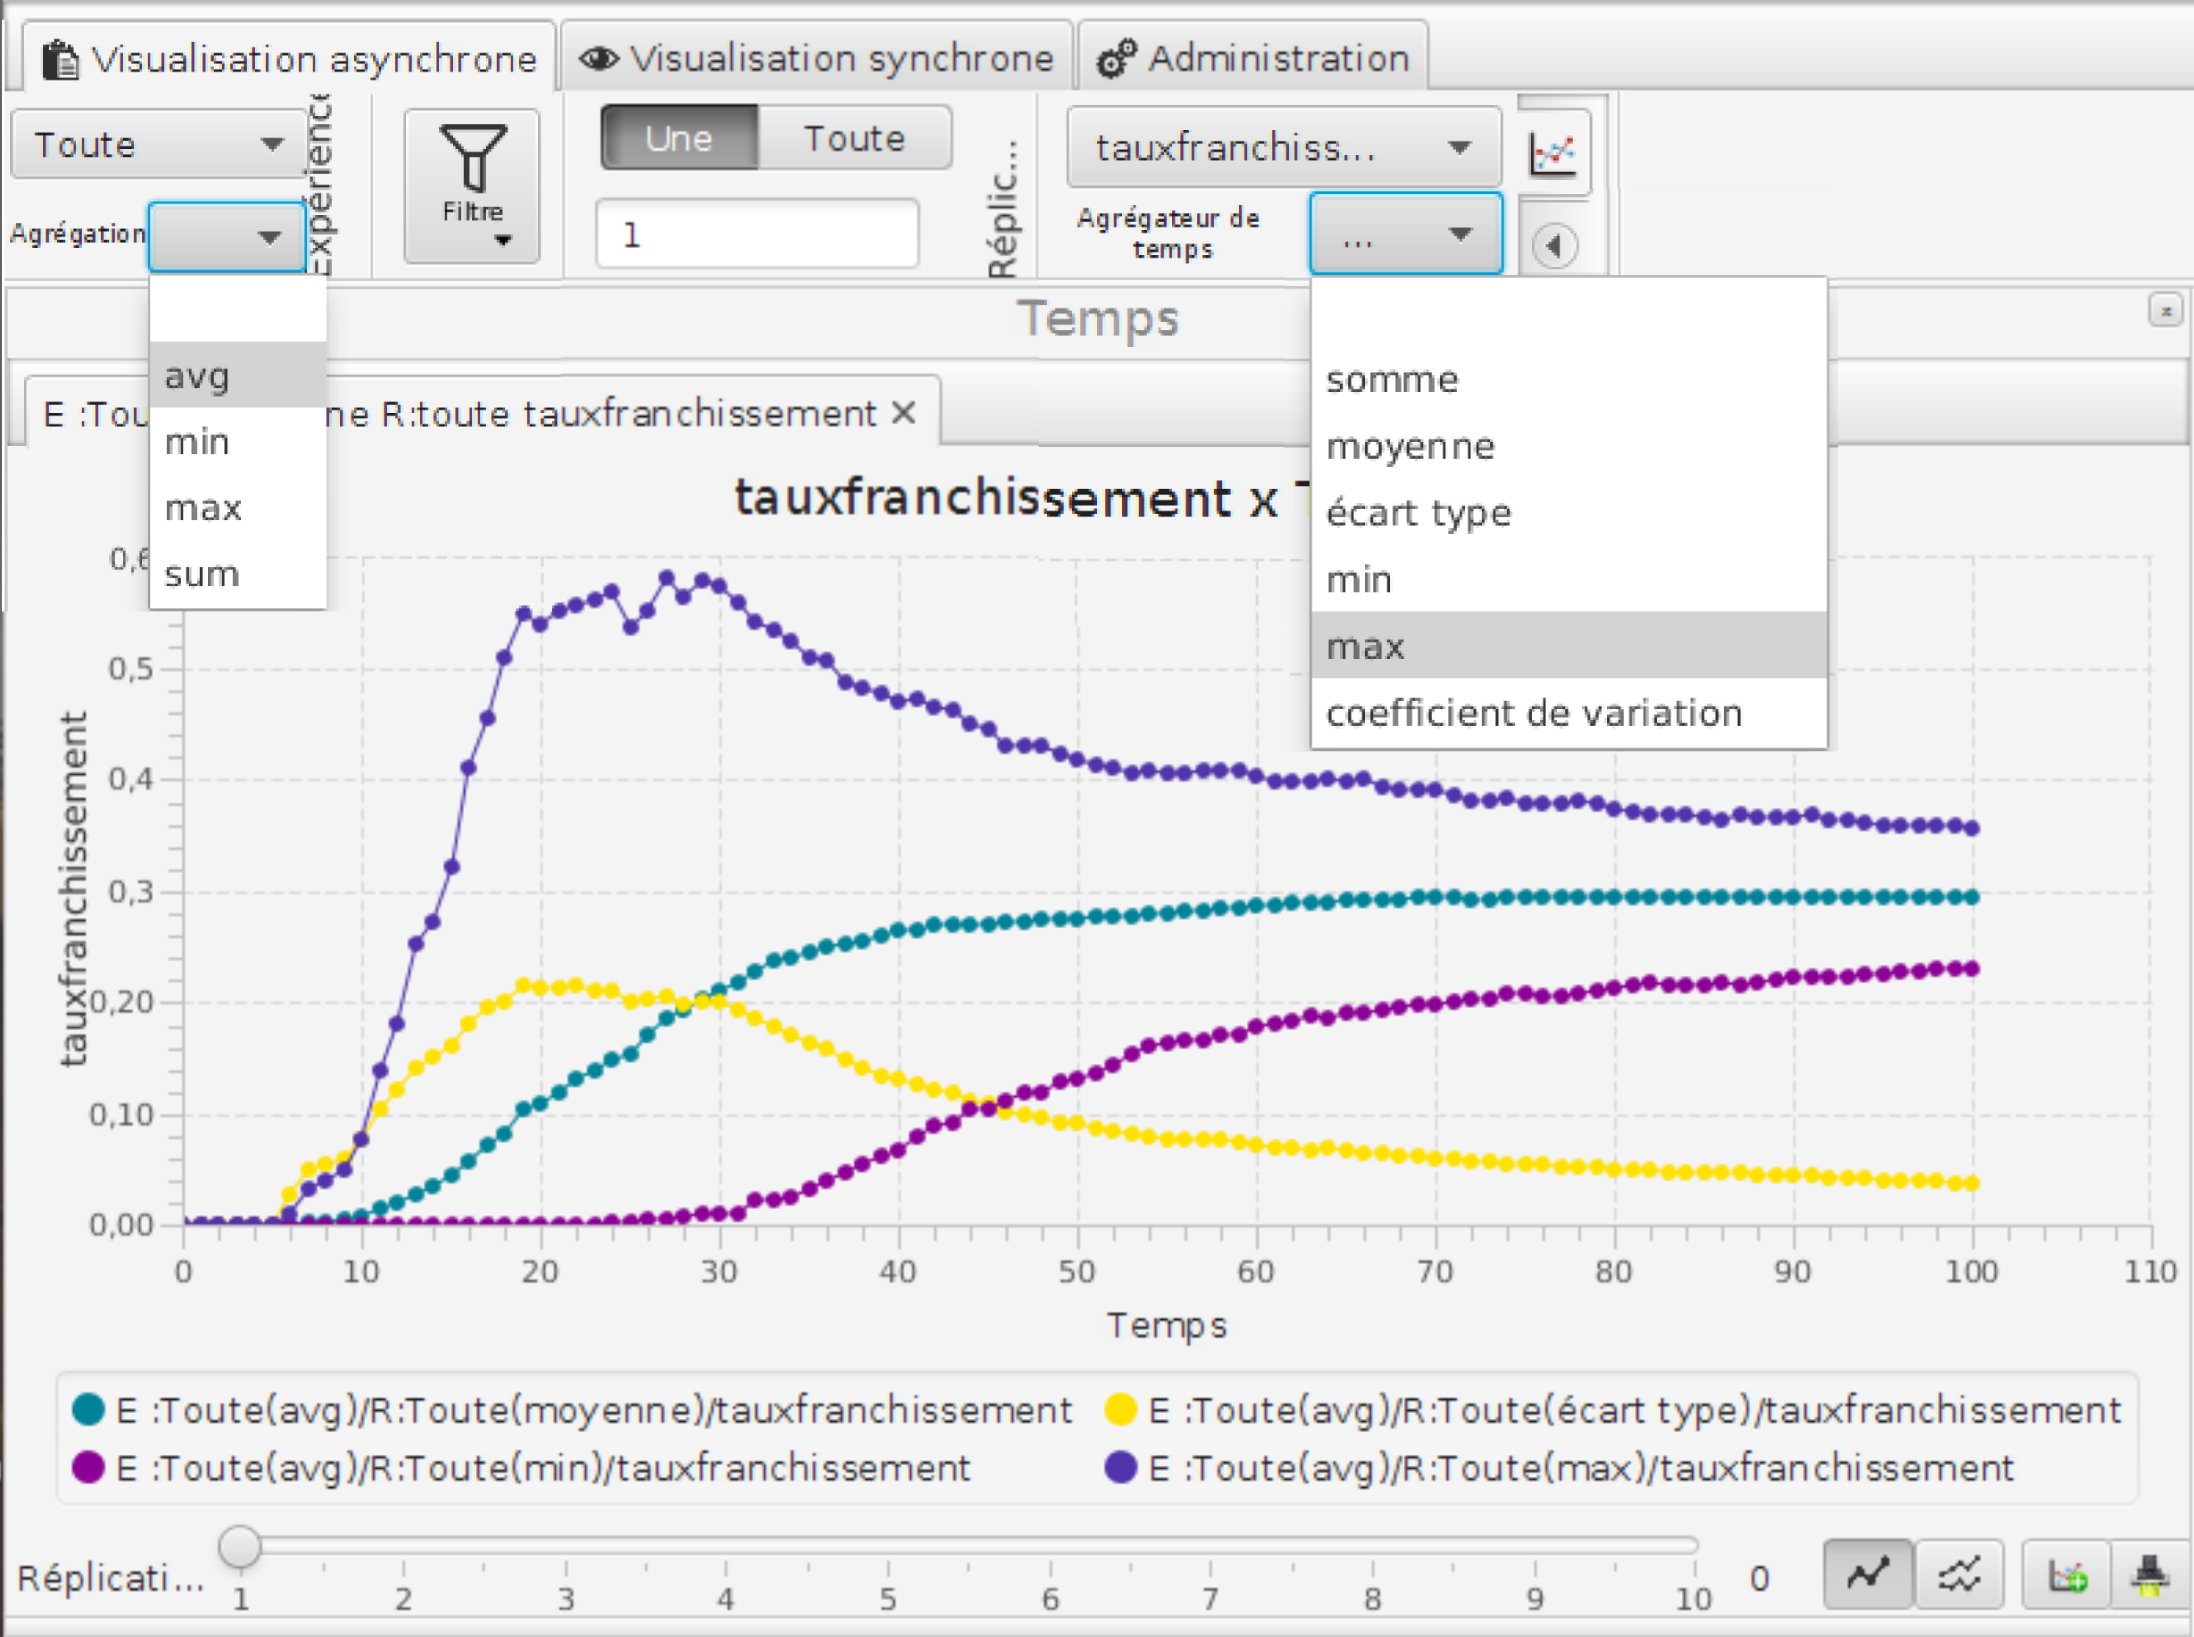
\includegraphics[width=.61\linewidth]{img/visuagent_agregations.png}}
	\captionsetup[subfloat]{width=.33\linewidth}
	\subfloat[][Deux cas théoriques d'évolution spatio-temporelle très similaires mais non agrégables.]{\label{subfig:agreg-espace}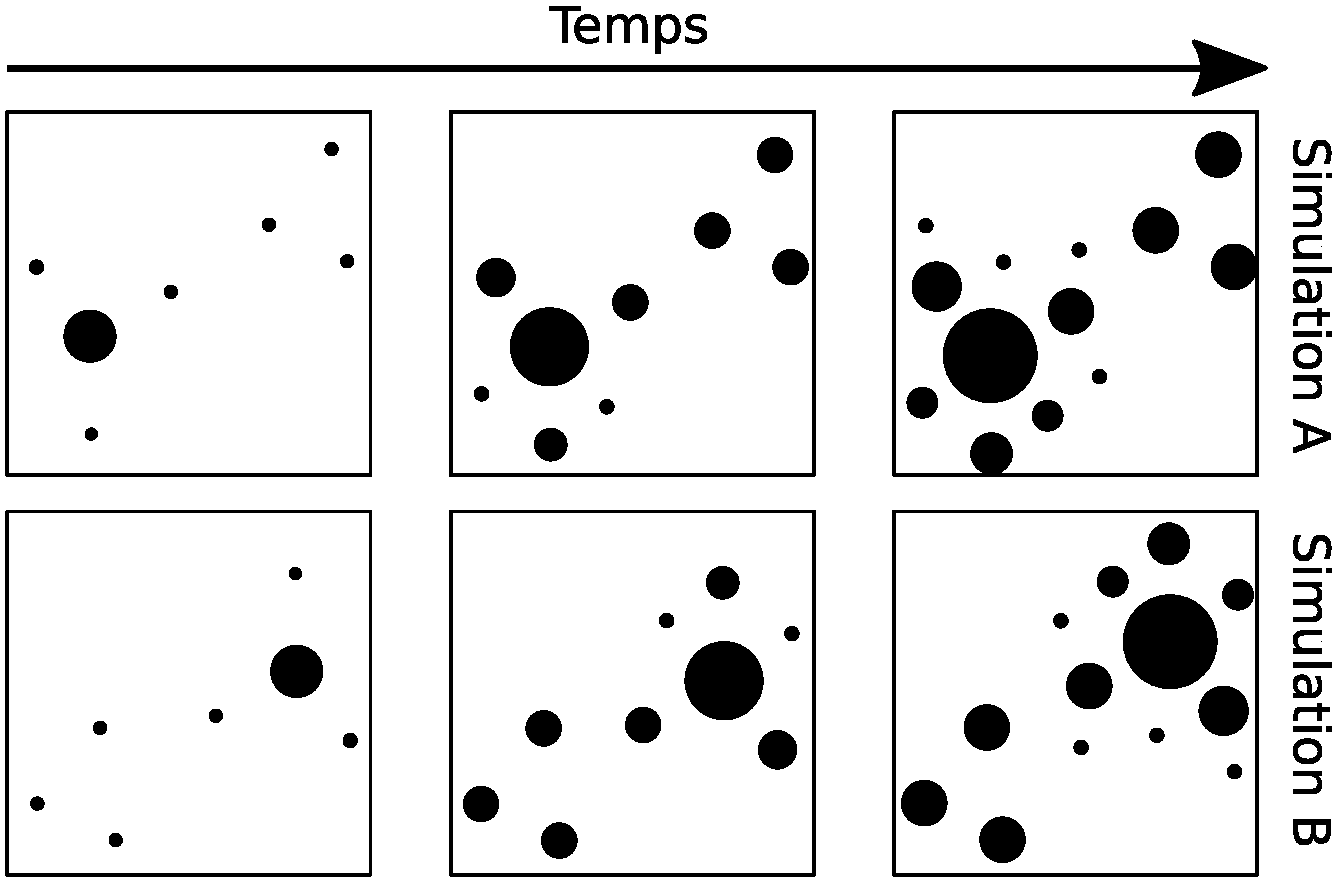
\includegraphics[width=.33\linewidth]{img/espace_theoriques.pdf}}
	\caption[Obstacles à l'agrégation de données pour la visualisation.]{Obstacles à l'agrégation de données pour la visualisation. Exemples tirés de \textcite{cura_visualisation_2020}}
\end{figure}


\noindent Dans le cadre de données de simulation, qui plus est quand l'espace est continu\footnote{
	Pour les données spatiales discrètes, par exemple quand l'espace prend la forme de cellules ou d'un maillage établi (régions, états\ldots), on peut mettre en place des systèmes graphiques de représentation de la forme des distributions d'une variable.
	Voir \textcite{ribecca_chart_2018} par exemple.
}, on ne peut réaliser d'agrégations des données sur la dimension spatiale que quand celle-ci est stable.
Dans un modèle comme SimFeodal, où l'espace est théorique, l'agrégation n'est pas possible car la répartition spatiale des agrégats, châteaux et églises change à chaque simulation.
La \cref{subfig:agreg-espace} illustre ce problème en présentant deux sorties de simulation théoriques, très proches en termes d'évolution, d'espacement, de structure globale, mais dont on ne peut tirer une représentation agrégée.
Pour le modélisateur, les deux alternatives sont donc ou bien de se contenter d'indicateurs numériques, agrégables, mais qui ne rendront pas correctement compte de la situation spatiale, ou bien de mener une observation de chacune des cartes correspondant aux différentes données produites par les réplications.


\subsection{Construction de connaissance par l'exploration visuelle d'un modèle}

Dans son Habilitation à Diriger des Recherches, \citeauteur{banos_pour_2013} décrivait neufs \og principes forts\fg{} de la modélisation \autocite[76--84]{banos_pour_2013}, dont le premier, \og Modéliser c'est apprendre\fg{}, était repris dans le titre de ce travail universitaire une fois publié \autocite{banos_modeliser_2016}.
Dans \textcite[\ppno~\hl{0--N}]{cura_visualisation_2020}, nous menons une comparaison point à point de ces neufs principes en les appliquant à la visualisation de données issues de modèles.
Nous reprenons ici quelques uns des arguments qui nous paraissent importants en termes de réflexivité, sur les potentiels gains de connaissances que l'exploration visuelle d'un modèle peut apporter.


\paragraph{La visualisation de modèle comme outil d'interdisciplinarité}
Les modélisateurs savent l’importance du dialogue dans la construction d’un modèle.
Dans son principe 2, \textcite[77]{banos_pour_2013} l’explicite ainsi :
	\og Le modélisateur doit avoir conscience du caractère fondamentalement limité de ses compétences.
	Ce qui peut être perçu comme une faiblesse est pour moi une force. Assumée, cette réalité mène naturellement à la collaboration.
	De manière très générale, je dirais même que modéliser un système complexe est un acte par essence collaboratif\fg{}.

\noindent La visualisation est un outil de communication au service de la transmission et de la diffusion d’un message.
Sans prise en compte de sa réception par ses lecteurs, le risque est important de concevoir un média peu compréhensible et donc peu utile.
Les retours du public visé sont donc importants, d’autant plus quand la visualisation doit aider à appuyer ou à transmettre un message complexe, requérant une expertise thématique, comme c’est souvent le cas dans le cadre d’un projet de modélisation.
Dès lors, le visualisateur ne peut agir seul, de la même manière que le modélisateur ne peut se contenter de sa seule expertise.

\noindent C'est d'autant plus vrai dans le cadre d'un modèle co-construit en interdisciplinarité.
Les différences de culture scientifique s'expriment aussi en termes de \og culture des données\fg{} (\textit{data litteracy}), c'est-à-dire par des habitudes et compétences hétérogènes en matière d'analyse et de visualisation de données.
Explorer visuellement un modèle, c'est avant tout se mettre d'accord sur ce que l'on veut observer, et ensuite sur la manière de le représenter.
Cette démarche, obligatoire, force à l'explicitation des détails techniques du modèle implémenté et de la manière précise dont les indicateurs de sortie sont obtenus, afin de minimiser le risque d'erreurs d'interprétation.

\noindent Par cette explicitation, ce dialogue, l'exploration visuelle d'un modèle force à la collaboration et, dans un cadre interdisciplinaire, à un réel partage de connaissances et de pratiques.
Ce faisant, l'exploration visuelle d'un modèle participe largement au rôle d'interface disciplinaire que la modélisation, en tant que telle, suscite.


\paragraph{L'exploration visuelle comme modélisation}
Simulation et visualisation sont des domaines scientifiques étudiés par des communautés disciplinaires très différentes et assez largement hermétiques.
Au sein même des réseaux francophones, les géographes se partagent par exemple entre différentes communautés.
La communauté de la géographie théorique et quantitative (colloques ThéoQuant et ECTQG, réseau S4, liens avec les Instituts des Systèmes Complexes\ldots) conçoit et développe des modèles depuis de nombreuses années, mais aussi des outils pour en explorer les sorties (voir \textcite{tannier:halshs-01003259} par exemple).
D'un autre côté, la communauté géomatique (colloques SAGEO, GDR CASSINI/MAGIS\ldots) s'intéresse notamment à l'exploration de données spatio-temporelles, à leur visualisation et modélisation, avec peut-être une entrée plus méthodologique que le premier ensemble.
Ces deux communautés communiquent peu, et cette situation n'est pas vraiment nouvelle\footnote{
	Il suffit de lire l'article qui introduit la publication des actes du colloque SAGEO 2005 pour s'en convaincre \autocite{josselin_presentation_2006}.
}.

\noindent Pourtant, que l'on reprenne les définitions de ce que sont les modèles\footnote{
	Chez \textcite{minsky_matter_1965} par exemple : \og To an observer B, an object A* is a model of an object A to the extent that B can use A* to answer questions that interest him about A.\fg{}
}, que l'on considère l'approche de modélisation graphique bien connue des géographes\footnote{
	Par exemple autour de la chorématique de \textcite{brunet1980composition}.
}, ou encore que l'on s'intéresse au rôle de la cartographie en géographie\footnote{
	Par exemple chez \textcite[246--247]{pinchemel_geographie_1979}, pour qui \og seule la représentation cartographique fait ressortir les organisations géographiques, les structures et les systèmes géographiques.
	La carte, le langage cartographique apparaissent aussi comme l'expression, comme le révélateur privilégiés de la géographie.
	La pensée géographique se lit dans les représentations cartographiques\fg{}.
}, il est difficile de ne pas voir dans la représentation graphique une certaine forme de modélisation de phénomènes sociaux ou spatiaux.
L'exploration visuelle, composée d'une succession de compositions graphiques que l'on raffine, transforme et dont on change le point de vue, est alors en tout point similaire au processus de construction d'un modèle de simulation \autocite{andrienko2018viewing}.

\noindent L'exploration visuelle n'est donc pas un processus isolé, particulier, mais peut alors s'inscrire dans les mêmes cadres théoriques et méthodologiques que la modélisation en tant que telle.
L'évaluation des outils et types de représentation joue par exemple un rôle essentiel et de premier plan dans les enjeux actuels rencontrés par les communautés scientifiques des \textit{visual analytics}, de l'interface homme-machine (IHM) ou encore de la visualisation de données (\textit{dataviz}, \textit{InfoVis}\ldots).
Il faudrait ainsi, dans l'absolu, mener une véritable évaluation de la méthode d'évaluation des modèles.
Dans le cadre de ce travail de thèse, nous n'avons pas poussé l'analyse jusque là, mais c'est un enjeux qui nous semble extrêmement important, pour être en mesure de qualifier et de comparer différentes méthodes d'évaluation, visuelles ou non, des modèles de simulation.

\paragraph{Visualiser, c'est apprendre}
Tout au long de son texte, \textcite{banos_pour_2013} met en avant un intérêt majeur (principe 1) à la modélisation : \og modéliser c'est apprendre\fg{}, principe qu'il reprend d'ailleurs comme titre pour la version publiée de ce travail universitaire \autocite{banos_modeliser_2016}.
Il explicite ce parti pris en inscrivant la modélisation dans une démarche itérative et abductive : \og
Modéliser est en effet un processus fondamentalement itératif qui -- et ce d'autant plus s'il est guidé par un principe d'abduction -- implique une interaction forte entre le modèle développé et la vision progressivement construite du phénomène en question
\fg{} \autocite[77]{banos_pour_2013}.
Il nous semble que le processus itératif mentionné caractérise la modélisation en général, ne s'exprimant pas plus dans une visée abductive -- que \textcite{livet2014diversite} associent aux modèles KISS par exemple -- que dans des modèles plus empirico-inductifs (ou déductifs) tels que les modèles KIDS.
L'itération est, nous semble-t-il, au cœur de toute démarche de modélisation, que celle-ci aille des hypothèses aux concepts, des données aux hypothèses, ou encore alterne entre les trois. 

\noindent L'exploration visuelle de modèles s'inscrit elle aussi dans une logique très comparable, en favorisant également cette posture itérative et abductive \autocite[\ppno~239--240]{banos2005voie}, présente dès les fondements de l'analyse exploratoire de données.

\paragraph[Ccl : Modélisation et visualisation]{}
Dans le cadre d'une activité de modélisation, la visualisation permet, on l'a vu, des allers-retours thématiques et méthodologiques entre modélisateurs et thématiciens, mais doit aussi s'adapter aux différentes évolutions du modèle :
	les modifications des sorties, des mécanismes, de l'ordonnancement etc. ont des conséquences en matière de visualisation, puisqu'elles affectent les données sur lesquelles celles-ci se fondent.
Quand bien même les données issues du modèle ne seraient pas amenées à évoluer, on peut concevoir la réalisation d'un processus de visualisation ou d'exploration visuelle dans les mêmes termes que le processus de modélisation \autocite{andrienko2018viewing}.
La visualisation de données issues du modèle est donc en elle-même un processus itératif, et permet de plus de renforcer cette itération en permettant au modèle d'évoluer à mesure que les visualisations éclairent sa compréhension.
L'exploration visuelle permet donc de gagner en compréhension sur le modèle, son objectif premier, mais aussi sur le système modélisé :
	en inscrivant le processus de modélisation-visualisation dans une boucle de rétroaction, on aboutit sur de nouvelles connaissances à propos du système-cible (\cref{fig:schema-va}).
Comme le résume \textcite{victor_simulation_2009} à propos de l'exploration visuelle, interactive dans son cas, de modèles : \og Model, Watch, Learn\fg{}.

\begin{figure}[H]
	\centering
	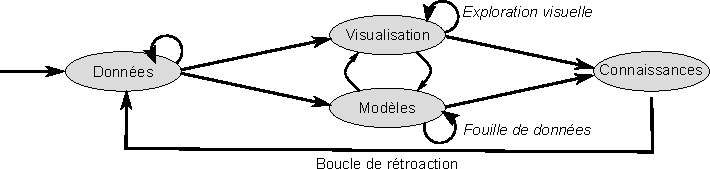
\includegraphics[width=\linewidth]{img/schema_keim.pdf}
	
	\caption[Itérations entre modèles et visualisations pour enrichir les connaissances.]{Itérations entre modèles et visualisations pour enrichir les connaissances, traduit d'après \textcite[fig.~1, p.~156]{keim_visual_2008}.}
	\label{fig:schema-va}
\end{figure}


\subsection{Comment passer de l'exploration à la validation ? Quelques perspectives \label{subsec:perspectives-validation}}

Dans le \hl{chapitre 3}, on définissait et décrivait les différents enjeux et méthodes de l'évaluation de modèle.
Notre approche, sur lesquels les paragraphes précédents constituent quelques retours, s'ancrait profondément dans une approche exploratoire et graphique, que nous dénommions \og évaluation visuelle\fg{}.
Au vu des très nombreuses étapes d'évaluation recommandées (cf. \hl{figures 3.2 et 3.3 du chapitre 3}), la question d'une évaluation plus systématique des modèles se pose tout de même.
On notait ainsi dans le chapitre 6 (cf. \hl{résultats}) que l'incertitude et l'incomplétude des données thématiques, empiriques, empêchait de pousser plus avant le raffinement du calibrage et de l'évaluation de SimFeodal.
Dans les paragraphes suivant, nous proposons quelques pistes pour améliorer les connaissances sur le modèle, et notamment sur ses qualités en termes de robustesse et de généricité.

\paragraph{Validation interne : quelques pistes pour une exploration plus systématique}
Une première piste, plusieurs fois évoquées auparavant, tient à l'usage de méthodes d'exploration de modèle plus automatisées et systématiques.
Ces méthodes, relatives à de la validation interne (cf. \hl{chap 3}), permettent d'obtenir une compréhension plus globale et fine à la fois du modèle.
Dans la description de l'analyse de sensibilité de SimFeodal (\hl{chap 6.2}), on précisait que nous nous étions restreint à une analyse de type \og one factor at a time\fg{}, sans faire covarier les valeurs de paramètres.
Dans le cadre d'un modèle véritablement complexe, qui plus est doté de très nombreux paramètres qui conditionnent des mécanismes dont l'interaction est importante\footnote{
 Voir par exemple les paramètres agissant de manière contre-intuitive, \hl{6.2.3}.
}, il est évident que modifier chaque paramètre indépendamment des autres n'esquisse qu'une faible part de la variabilité que ceux-ci peuvent avoir sur les sorties du modèle.
Au contraire, une analyse de sensibilité croisée, testant automatiquement différentes combinaisons de paramètres, permettrait de connaître de manière plus approfondie la gamme de réactions du modèle à des changements de paramètres.

\noindent Le principal défaut des méthodes croisées tient aux risques d'explosion combinatoire, qui plus est avec un modèle doté de très nombreux paramètres.
Plutôt que de mener des analyses sur le plan complet, des méthodes ont été mises au point pour explorer l'espace des sorties d'un modèle.
Celles-ci permettent, en suivant des heuristiques, de déterminer des sous-ensembles de valeurs à tester, que ce soit en suivant des logiques d'algorithmes génétiques \autocite{schmitt_half_2015,rey-coyrehourcq_plateforme_2015}, des logiques de recherche d'optima locaux \autocite{schmitt_modelisation_2014, reuillon_new_2015} ou encore de recherche de motifs dans les sorties \autocite{cherel_beyond_2015}.

\noindent Ces méthodes sont extrêmement prometteuses et utiles car elles permettent d'explorer la vaste étendue des comportements d'un modèle en restreignant fortement le nombre de simulations nécessaires.
Elles requièrent toutefois la définition d'un faible nombre d'indicateurs de sortie, quantitatifs, sur lesquels les différents algorithmes pourront s'appuyer pour définir les valeurs de paramètres à échantillonner.
De plus, l'exemple de l'exploration de l'espace des paramètres du modèle SimpopLocal \autocite{schmitt_modelisation_2014} avec l'une de ces méthodes, \og Calibration Profile\fg{} \autocite{reuillon_new_2015} montre que pour ce modèle KISS, doté de seulement 5 paramètres, 100 000 heures de calcul machine ont été nécessaires\footnote{
	Réduites à 15 jours de calcul en utilisant les possibilités de calcul distribué mises à disposition par l'infrastructure de calcul intensif EGI.
}.
Sur un modèle moins parcimonieux, le temps nécessaire serait immense, sans même compter la consommation électrique correspondante.
Pour SimFeodal, l'apport de connaissances et le raffinement de l'évaluation justifient-ils un tel coût ?
Il nous semble que ces méthodes sont strictement inapplicables en l'état actuel du modèle, mais avec un important travail de réduction des paramètres et de quantification et synthèse des indicateurs de sortie, elles pourraient apporter des connaissances intéressantes sur le modèle et aider à le rendre plus générique.
Enfin, vu la complexité des données que ces méthodes peuvent produire, il serait à nouveau utile de mener des phases d'exploration et d'interprétation, visuelle notamment, de leurs résultats.
Quelle que soit la complexité et l'efficacité des méthodes de fouille automatique de données ou de modèles, il semble inévitable d'avoir à en mener des analyses de plausibilité visuelle pour en vérifier ou en comprendre les conclusions.
Une plateforme telle que SimEDB serait entièrement adaptée à l'exploration visuelle des sorties de ces modèles de modèle.

\paragraph{Validation externe : données empiriques et confrontation}
Une seconde piste concerne cette fois-ci la validation externe, c'est-à-dire l'évaluation du modèle au regard des connaissances empiriques dont on dispose sur la période et la région d'étude.
Cette approche, très classique, correspond à la \og statistical validation\fg{} (\hl{fig 3.2}) ou \og output validation\fg{} (\hl{fig. 3.3}).
Dans le cas de SimFeodal, nous pensions au départ de ce travail de thèse mener une confrontation, point par point, entre les nombreuses données archéologiques qui ont été compilées pour la Touraine (\textcite{rodier_modelisation_2010} par exemple), et les indicateurs correspondants du modèle.
Très vite, on a pourtant réalisé qu'il serait vain de vouloir comparer les données issues d'un modèle de simulation descriptif et théorique, à des données empiriques lacunaires et d'un ordre de généricité bien moindre.
Les degrés de précision de ces deux pendant des données à confronter sont ainsi trop différents pour être véritablement comparables.

\noindent Hors de la confrontation directe de l'ensemble des sorties du modèle avec les données empiriques correspondantes, on retrouve deux approches complémentaires (voir la \cref{fig:JIG}) qui pourraient être intéressantes en perspectives d'évolution du modèle.
Ces deux approches partent de données historiques et archéologiques pour concevoir des modèles, statistique dans un cas \autocite{gravier_deux_2018} et graphique dans l'autre \autocite{nahassia_formes_2019}.

\begin{figure}[H]
	\centering
	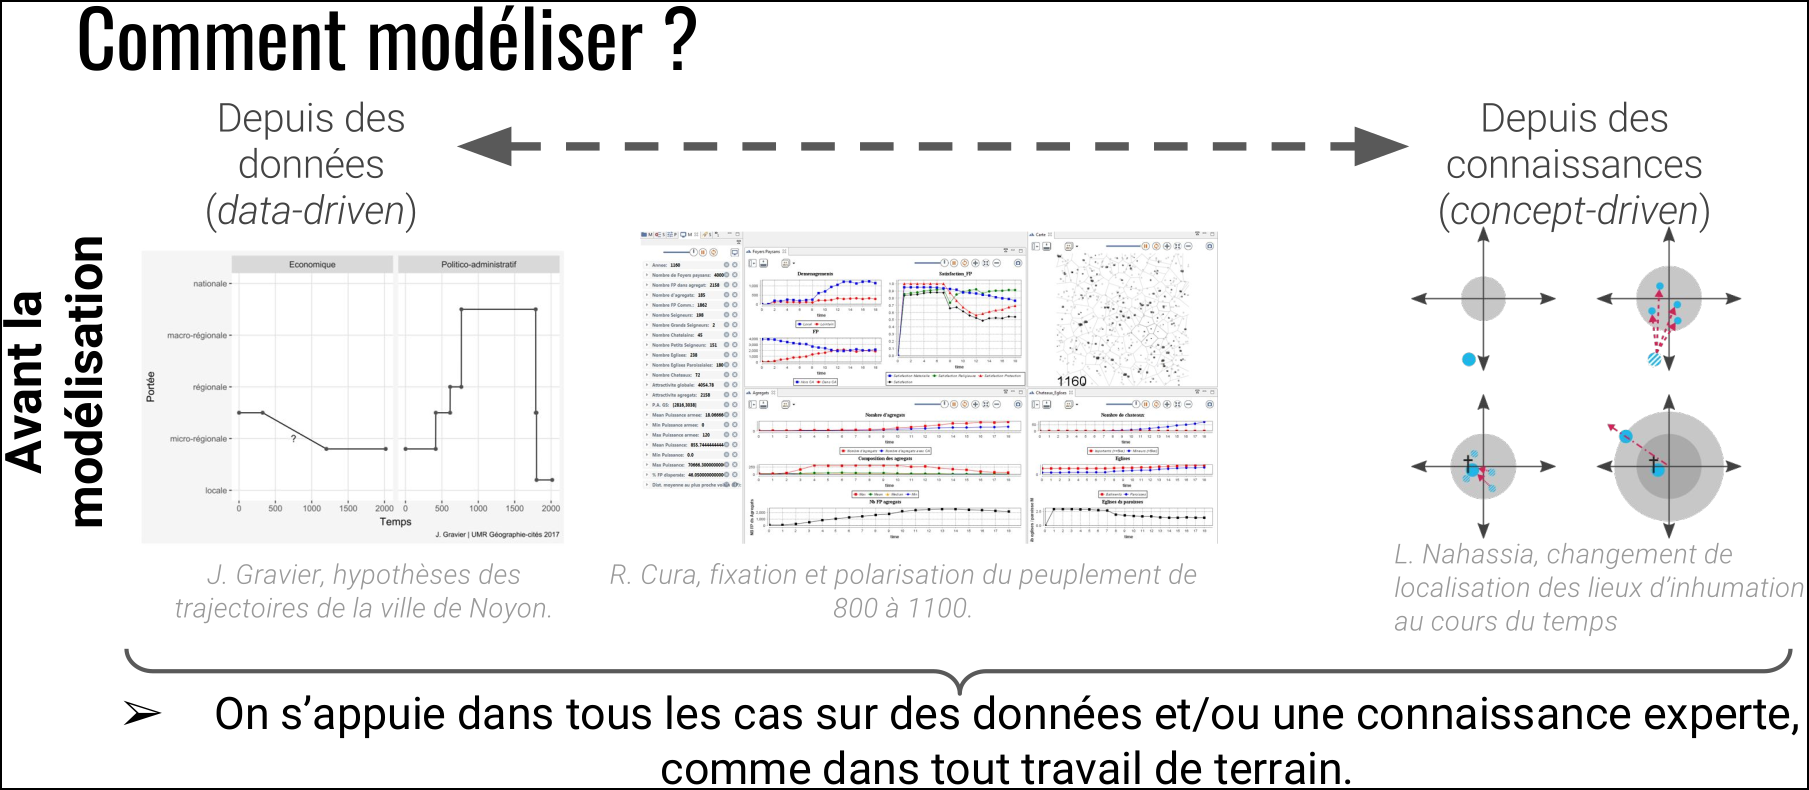
\includegraphics[width=\linewidth]{img/types_modelisation_JIG.png}
	
	\caption[Trois approches de modélisation différentes de processus sociaux et spatiaux sur le temps long.]{Trois approches de modélisation différentes de processus sociaux et spatiaux sur le temps long \autocite{cura:halshs-02296147}.}
	\label{fig:JIG}
\end{figure}

\noindent \textcite{gravier_deux_2018} prend appui sur la constitution de bases de données harmonisées, d'une résolution très fine et tendant vers l'exhaustivité.
Elle mobilise ces données afin d'estimer statistiquement, entre autre, l'importance relative de différents lieux au regard de leurs relations et interactions.
La diversité des sources archéologiques et historiques est donc importante, mais au service d'une seule question thématique, et l'hétérogénéité thématique des données est donc assez restreinte.
L'étendue spatiale de la zone modélisée est importante, mais comme le questionnement thématique est très circonscrit, la qualité des données permet d'y apporter une réponse robuste.
Appliqué à SimFeodal, il s'agirait donc d'aller vers la constitution de bases de données cherchant l'exhaustivité et la précision, sur une diversité de questionnements plus restreinte :
	s'intéresser à des phénomènes très spécifiques, mais en mener une collecte et une analyse très poussée.
On pourrait par exemple chercher des données correspondant à l'un des indicateurs du modèle, l'évolution de la distance moyenne à l'église paroissiale la plus proche par exemple.
En se gardant d'incorporer ces données lors du calibrage du modèle, on pourrait alors constituer un jeu de données de test, composé de ces données empiriques précises, par lequel éprouver les données de sortie du modèle.

\noindent À l'opposée, \textcite{nahassia_formes_2019} effectue une modélisation graphique à partir de connaissances théoriques, et éprouve les hypothèses qui en découlent, relative par exemple aux évolutions de localisation de différents types de structures intra-urbaines.
L'évaluation de ses modèles graphiques consiste à confronter ces hypothèses aux riches données dont elle dispose pour la ville de Tours.
La réduction de la masse de données ne se fait pas en restreignant la diversité thématique, mais en limitant le cas d'étude à une unique ville, point de départ d'une méthodologie reproductible et généralisable.
En nous inspirant de cette approche, on pourrait par exemple chercher à collecter le maximum d'informations et de données sur une zone à l'étendue restreinte (une paroisse par exemple).
Comme pour l'exemple précédent, on pourrait alors utiliser la correspondance spécifique de l'une des sous-régions modélisées comme critère d'ajustement.
Cette réduction pourrait aussi être temporelle, en ne considérant comme \og crible intermédiaire\fg{}, comme dans la méthode POM \autocite{grimm_pattern-oriented_2005,grimm_pattern-oriented_2012}, que l'accomplissement des faits stylisés choisis sur une partie limitée de la temporalité totale du modèle.

\noindent Dans les deux cas, ces possibilités d'évolution de l'évaluation du modèle procèdent de manière finalement assez similaire face à un problème commun.
Il n'est en effet pas possible d'obtenir des éléments empiriques quantifiés sur l'ensemble de la diversité des processus modélisés, sur l'ensemble de la région et sur l'ensemble de la période.
Une solution serait donc d'ajuster le modèle sur des sous-ensembles témoins de l'une ou plusieurs de ces dimensions (thématique, spatiale, temporelle).
Cette approche est fréquemment utilisée pour les modèles statistiques prédictifs (scénarios démographiques et climatiques entre autre), qui peuvent par exemple avoir pour point de départ temporel une période relativement récente, et où on cherche à ce que les \og rétro-prédictions\fg{} collent aux données empiriques déjà connues au moment de la création du modèle.


\paragraph{Validation croisée : désancrer le modèle pour en évaluer la généricité}\label{par:validation-croisee}
Une dernière piste, évoquée\noindent  dès les prémices de ce travail de thèse, consisterait à mener une évaluation par le biais de \og scénarios régionaux\fg{}.
Dans le chapitre précédent, nous présentions une analyse de scénarios thématiques qui nous paraissent intéressants au regard des questionnements des archéologues et historiens de notre groupe de travail.
Ces scénarios sont plausibles et doivent aider aussi bien à tester la robustesse du modèle face à des changements de valeurs de paramètres nets qu'à évaluer la réaction des interactions entre mécanismes dans des contextes thématiques légèrement différents (augmentation de la part des foyers paysans dépendants -- serfs et esclaves --, hypothèses de croissance démographique\ldots).

\noindent Les scénarios que nous entendons maintenant pour participer à l'évaluation du modèle seraient plutôt des scénarios régionaux, c'est-à-dire qu'ils viseraient à adapter les valeurs calibrées du modèle à d'autres contextes spatiaux et temporels.
SimFeodal est un modèle qui se veut générique à l'Europe du Nord-Ouest, mais a été calibré sur une région particulière, la Touraine.
En désancrant le modèle, c'est-à-dire en l'adaptant à une autre région dotée de paramètres différents, on pourrait ainsi procéder à une sorte de validation croisée (\textit{cross validation}).
Si le modèle, une fois ses \textit{inputs} et paramètres de contexte adaptés à la description d'une autre région, produit des résultats plausibles pour les experts thématiciens de cette autre région, alors on peut penser que SimFeodal réussit à reproduire les faits stylisés recherchés de manière plus robuste qu'initialement.
On sait que les faits stylisés modélisés dans SimFeodal sont génériques à l'Europe du Nord-Ouest, mais selon des rythmes et des proportions propres à chaque région.
Si l'on prend l'exemple d'un diocèse montagnard, on pourrait alors diminuer les différents seuils de distance paramétrés selon des connaissances d'experts, ici pour tenir compte du relief plus difficile aboutissant à temps de parcours augmentés.
Aboutirait-on à une concentration plus lente, moins nette, ou au contraire est-ce que ce processus serait accéléré et augmenté ?
En travaillant avec des spécialistes historiques de ces régions, on pourrait ainsi tester la validité des hypothèses du modèle sur leurs propres terrains d'expertise.

Dans une temporalité ultérieure à celle du présent travail, un séminaire est déjà prévu et vise à éprouver SimFeodal sur d'autres régions dans lesquelles les historiens trouvent des similarités générales de changement de structure spatiales -- ou au contraire des processus très différents -- et sur lesquelles les sources empiriques paraissent suffisantes (Normandie, Champagne, Lorraine, Alsace, Flandre, Poitou, Provence, Quercy\ldots).
Là encore, pour le dialogue interdisciplinaire et inter-régional, l'utilisation de représentations graphiques interactives comme interface entre les chercheurs présenterait sans doute les mêmes avantages discutés dans ce travail de thèse.


\subsection{Conclusion : Pour un recours systématique à la visualisation dans l'analyse de modèles}
Dans cette partie, nous somme revenus sur les nombreux bénéfices que l'analyse exploratoire visuelle, largement reconnue vis-à-vis des données classiques, a pu apporter dans le cadre de notre expérience interdisciplinaire de conception et de développement de modèle, dont SimFeodal est est le résultat.
Plus largement, ce retour d'expérience nous conforte dans l'idée que la modélisation pourrait profiter d'un recours plus systématique à l'analyse visuelle des données produites.
Cela nous semble résonner d'autant plus dans le cas des modèles spatiaux tant la pratique de la représentation graphique est ancrée dans la culture disciplinaire des géographes.
Nous ne pouvons pourtant, parallèlement, que constater la faiblesse de la production (carto)graphique dans le domaine de la modélisation \autocite[Introduction]{cura_visualisation_2020}, quand bien même les plateformes de simulation multi-agents rivalisent de possibilités en ce sens.

\noindent Afin d’encourager les modélisateurs à s’emparer de la question de la visualisation, nous avons montré que tout au long du cycle de développement d'un modèle, la visualisation peut aider le modélisateur et les spécialistes thématiciens qui l’entourent  :
dès sa conception, en participant à la co-construction et au travail collaboratif (la visualisation comme interface interdisciplinaire, comme formalisme d'explicitation des composantes et sorties d'un modèle\ldots) ;
mais aussi, une fois le modèle implémenté, comme outil d'évaluation et support à une potentielle validation des modèles (validation interne, méthodes d'exploration automatiques et validation croisée).

\noindent Pour que ces apports soient complets et utiles à tous, le transfert disciplinaire ne peut être à sens unique : là où les géographes peuvent bénéficier des recherches en visualisation de données, celles-ci gagneraient aussi à affronter les problématiques propres aux données issues modèles de simulation géographiques que nous avons esquissé (\cref{subsec:genericite-donnees-simul}).
Pour paraphraser \textcite[76]{banos_pour_2013}, \og il ne suffit pas de mettre en contact des disciplines pour que l’interdisciplinarité émerge.
La pluridisciplinarité s’en contente facilement, mais l’interdisciplinarité implique des interactions entre disciplines et par conséquent une nécessaire acculturation [...]
Donner les moyens aux géographes et, au delà, aux chercheurs en sciences humaines et sociales, de devenir plus autonomes dans leur démarche de [visualisation\footnote{
	\og Modélisation\fg{} dans le texte original.
}] va [aussi] dans ce sens\fg{}.


\clearpage
\let\orisectionmark\sectionmark
\renewcommand\sectionmark[1]{}%
\section{Retours sur la co-construction d'un modèle de simulation descriptif}
\orisectionmark{Retours sur la co-construction d'un modèle de simulation descriptif}
\let\sectionmark\orisectionmark

Tout au long de ce travail de thèse, nous avons choisi de tenir -- et essayé de maintenir -- un positionnement réellement collectif et collaboratif.
Nous souhaitions, comme annoncé dans \hl{le chapitre 1}, co-construire un modèle plutôt que de construire un modèle \og pour\fg{} des collègues historiens et archéologues.
Le travail de modélisation qui a abouti à SimFeodal a été initié au sein du projet ANR TransMonDyn, avant le début formel de ce travail de thèse.
Ce travail de modélisation n'est pas achevé : son cadre dépasse celui de la thèse, et des projets en cours voire à l'état d'initialisation sont encore prévus pour faire vivre ce modèle et la démarche qui en a animé la construction, l'évaluation et l'utilisation.
Le rendu de ce manuscrit est l'occasion de réaliser un point d'étape dans ce processus de modélisation qui s'inscrit résolument sur la longue durée, relativement à l'échelle de la recherche.

Ce point d'étape, présenté sous la forme d'un retour d'expérience structuré plutôt que chronologique, me pousse à réaliser un bilan réflexif sur les conditions souhaitées mais aussi concrètement réalisées de construction du modèle SimFeodal.

Dans le \hl{chapitre 1} (1.4.1), j'ai présenté l'approche ComMod (Modélisation d'accompagnement) en identifiant ses différences avec la démarche que nous souhaitions emprunter dans cette expérience de modélisation collective.
Les points de divergence présumés étaient notamment la volonté forte d'aller jusqu'au modèle implémenté dans notre projet, ce qui n'est pas systématiquement fait dans l'approche ComMod, de même que la séparation entre \og animateurs\fg{} et \og participants\fg{} dans l'approche ComMod, qui mène une distinction des rôles que nous souhaitions effacer dans un processus de co-construction.
Dans cette partie, je reviens sur ces deux points de divergence prévus, en discutant de leur validité réelle \og \textit{a posteriori}\fg{}\footnote{
	Cet \textit{a posteriori} est en fait temporaire, comme indiqué plus haut.
} de cette expérience de co-construction de modèle.
Dans un retour sur les deux premiers chapitres, qui présentaient SimFeodal comme un modèle exploratoire et descriptif et le justifiaient, je pourrai alors discuter du positionnement final du modèle, ce qui permettra aussi de revenir sur l'évolution de ce positionnement.


\subsection{Un retour d'expérience critique sur l'usage de modèles de simulation descriptifs : les limites de l'implémentation}

L'expérience constituée par ces nombreuses années de travail sur le modèle SimFeodal pourrait aller dans le même sens que l'approche ComMod, au regard des nombreuses limites qui me semblent désormais apparentes quant à l'utilité du modèle implémenté en lui-même.
Dès le départ, nous avions fixé un rôle exploratoire au modèle, en en faisant avant tout un support à la pensée.
Nous ambitionnions cependant de pouvoir tester les hypothèses thématiques, non pas pour les (in)valider, mais pour être en mesure de vérifier s'il était possible que ces hypothèses puissent être nécessaires et suffisantes pour reproduire les processus empiriques étudiés.

\paragraph{Quel usage pour un modèle de simulation descriptif et exploratoire ?}

Après coup, cette ambition ne me paraît pas entièrement -- ou pas encore -- satisfaite.
Au delà de l'équifinalité, c'est-à-dire du fait qu'une infinité potentielle de modèles de toutes formes permettent de reproduire les mêmes données ou motifs, il me semble ainsi que le choix d'un modèle exploratoire et descriptif augmente les biais possibles quant à l'éventuelle utilisation d'un modèle en vue de prouver un phénomène.
En effet, dans un modèle, chaque mécanisme peut être conçu, puis implémenté de plusieurs manières différentes.
En multipliant les mécanismes, on augmente d'autant le nombre de solutions alternatives possibles, et on augmente exponentiellement le nombre de combinaisons potentielles résultants de ces alternatives possibles.
Dans un modèle statistique, à mesure que l'on ajoute des variables, on augmente presque mécaniquement l'ajustement global du modèle aux données étudiées.
Même sans ajouter de variables explicatives, on peut renforcer l'ajustement d'un modèle quelconque en en complexifiant la formulation.
Par exemple, pour une même série de point que l'on chercherait à décrire par une régression polynomiale, plus le degré de ce polynôme augmente, plus l'ajustement est amélioré lui aussi.
Est-ce pour autant que la variable explicative est plus valide qu'avec une régression polynomiale de degré 1, c'est-à-dire une régression linéaire ?

Dans un modèle très stylisé où seuls quelques mécanismes sont présents, on est capable d'affirmer que la conjonction de ces mécanismes est un candidat potentiel à l'explication, voire d'éliminer d'autres candidats potentiels à l'explication.
Dans un modèle plus descriptif, l'accumulation de choix me semble rendre plus difficile cette affirmation.
Dans l'exemple de SimFeodal, on cherchait à pouvoir affirmer que la polarisation et la hiérarchie du système de peuplement pouvaient être expliquée par des dynamiques liées d'émiettement des pouvoirs, d'augmentation de la violence et d'augmentation de l'encadrement religieux.
Dans l'état actuel du modèle, le risque est que ce soient les conditions particulières d'implémentation du modèle conceptuel, c'est-à-dire la somme des choix techniques d'implémentation, qui aboutissent en un modèle dont les résultats sont satisfaisants.

\paragraph{Validité interne d'un modèle complexe.}
Ce constat est aggravé par la nature complexe (en termes de complexité algorithmique) de l'implémentation informatique, qui en rend nécessairement l'évaluation interne plus difficile.
Avec un modèle composé de plus de 2 000 lignes de code comme SimFeodal, le risque d'erreur -- méthodologiques ou techniques -- est infiniment plus important que sur un modèle-jouet composé de quelques dizaines de lignes de code.
Lors du paramétrage de SimFeodal, de très nombreuses erreurs ont été détectées et corrigées : parfois le code ne correspondait méthodologiquement pas au mécanisme tel qu'il avait été défini, parfois, le choix de telle ou telle fonction informatique ne retournait pas le résultat décrit dans la documentation, parfois, un mécanisme était court-circuité par un autre, etc.
Il est habituel, et presque attendu, qu'un programme informatique contienne des erreurs ou \textit{bugs}, mais en complexifiant ce programme, on augmente fortement ce risque d'erreur.

Ces erreurs sont le plus souvent de la responsabilité de ceux qui implémentent du modèle, mais parfois, elles dépendent aussi d'éléments difficiles à contrôler, telle que la présence d'erreurs au sein même des outils utilisés pour mener la modélisation.
C'est un risque inhérent à l'utilisation de plateformes de modélisation \og de recherche\fg{} : les développeurs de ces outils sont tout autant susceptibles de commettre des erreurs d'implémentation que les modélisateurs.
Ils en commettront sans doute moins proportionnellement qu'un géographe non informaticien, mais la complexité du code n'est pas du même ordre de grandeur non plus.
La plateforme de simulation Gama, par exemple, repose sur plus de 500 000 lignes de code.
Parmi celle-ci, la probabilité qu'il n'y ait aucune erreur est quasi-nulle, en dépit des très nombreux et réguliers \textit{commits} qui viennent justement corriger les \textit{bugs}.
Une bonne partie de ces \textit{bugs} sont en fait peu dommageables dans le cas de SimFeodal, pouvant porter sur des fonctions que nous n'utilisons pas, ou sur des conjonctions de cas non rencontrés dans notre modèle.
Pourtant, une erreur importante concernant l'ordonnancement des agents a été détectée et corrigée sur la plateforme Gama en mai 2016, qui était alors en version 1.7, c'est-à-dire jugée stable.
Cette erreur, survenue entre les version 3 et 4 de SimFeodal (cf. \hl{tableau des versions}) a eu des conséquences majeures sur les résultats du modèle, et une large partie des expériences réalisées précédemment a du être ré-exécutée pour en vérifier les sorties une fois le \textit{bug} corrigé.

Lors du passage du modèle conceptuel au modèle implémenté, il y a donc de fortes chances que des erreurs -- introduites lors de l'implémentation ou lattentes à la plateforme utilisée -- viennent invalider les résultats thématiques proposés à grâce au modèle.
Même dans un modèle parfaitement implémenté, l'équifinalité face aux choix techniques d'implémentation peuvent aussi largement restreindre la qualité démonstrative du modèle : ce ne sont pas les hypothèses intégrées dans le modèle qui pourront constituer des candidats à l'explication thématique.
Ces candidats à l'explication seront toujours dépendants de la manière dont le modèle est implémenté.

\paragraph{De l'importance de l'implémentation.}
Ce bilan n'est pas pour autant véritablement négatif.
Dans l'\hl{introduction générale}, je décrivais la simulation informatique comme un moyen de mener des expérimentations \textit{in silico} quand cela n'était pas possible \textit{in vivo}.
L'écart entre les deux, surtout quand on modélise des processus sociaux (spatiaux ou non) me paraît au final assez faible en matière de capacité de démonstration.
En expérimentation sociale, il est indispensable de chercher à identifier les biais potentiels d'une étude, et d'en estimer les effets pour parvenir à contrôler les paramètres d'une expérience.
En simulation informatique, ces biais sont aussi présents, sous la forme d'erreurs potentielles, et il est tout aussi difficile de les contrôler qu'en sciences sociales expérimentales.
Tous les biais décrits comme \og limites de l'implémentation\fg{} dans cette sous-partie me semblent donc au final assez banals et inhérents aux méthodes expérimentales, quel qu'en soit le support, informatique ou social.

Dans le cadre d'une démarche collective de modélisation, ces quelques limites ne remettent dans les faits aucunement en cause les principaux atouts introduits dans le \hl{chapitre 1}.
L'implémentation informatique du modèle a nettement renforcé le besoin d'explicitation des hypothèses introduites.
Plus le formalisme employé est précis et non ambigu (ce qui est le cas des formalismes informatiques et non des modèles \og rhétoriques\fg{} ou \og graphiques\fg{} évoqués dans l' introduction générale), plus son utilisation oblige à désambigüiser le discours.
En allant jusqu'à l'implémentation informatique, nous avons collectivement été amenés à trancher des centaines de choix, à expliciter à de multiples reprises le contenu de chacun des nombreux mécanismes, et donc à élaborer ensemble une compréhension partagée de ce modèle, sur l'ensemble des domaines qui le caractérisent.
De plus, un modèle de simulation descriptif est un outil dont la complexité permet aussi d'incessantes modifications, que ce soient des corrections ou des améliorations.
Un tel modèle constitue ainsi un support à la discussion dont la \og durée de vie\fg{} me paraît supérieure à celle d'un modèle plus simple, parce que les possibilités de raffinement sont nombreuses, ce qui contribue à inscrire la réflexion collective autour du modèle dans la durée.

\subsection{Quelle part effective du collectif dans la conception et l'implémentation du modèle ?}

Tout au long de cette thèse, j'ai insisté sur la dimension collective, de co-construction, qui a permis d'aboutir au modèle SimFeodal présenté dans ce manuscrit.
On pourrait objecter, au regard des \textit{commits} du modèle, que seules deux personnes ont effectivement apporté des modifications dans le dépôt logiciel.
En regardant plus en détail l'historique de ce dépôt, on pourrait même constater que Cécile \textsc{Tannier}, l'autre contributrice du dépôt, n'est intervenue \og que\fg{} dans de nombreuses modifications de la documentation du modèle.
Le code-source de SimFeodal n'a donc été implémenté, en tant que telle, que par moi seul.

Cela signifie-t-il pour autant que la volonté de co-construction globale, du modèle conceptuel jusqu'au modèle implémenté, n'a finalement pas été respectée ?
Avant de répondre à cette question, je crois important de justifier la décision de cette implémentation mono-participante, qui pourrait largement accréditer la distinction entre \og participant\fg{} et \og animateur\fg{} (ou \og implémenteur\fg{}, voir \hl{chap1, section 1.1.4 p. 26}).

\paragraph{Compétences spécifiques nécessaires pour l'implémentation d'un modèle de simulation.}
Le développement informatique d'un modèle de simulation demande des compétences particulières.
En premier lieu, des compétences méthodologiques, bien sûr, qui concernent la capacité à transcrire sous forme algorithmique les mécanismes et interactions exprimées dans un modèle conceptuel.
Ces compétences sont l'une des caractéristiques attendues d'un \og modélisateur\fg{}, et assez répandues dans les sous-domaines quantitatifs des sciences humaines et sociales.
En second lieu, au-delà de ces compétences méthodologiques, le développement d'un modèle de simulation requiert aussi des compétences techniques assez spécifiques et détaillées.
Les algorithmes et fonctions doivent en effet nécessairement être \og implémentés\fg{}, informatiquement, dans un langage de programmation.
Cette implémentation demande donc d'effectuer du \og développement informatique\fg{}, et à ce titre, exige la connaissance de ces langages de programmation.
Dans le monde de la simulation à base d'agents, les différentes plateformes disponibles mobilisent de nombreux langages de programmation.
Dans une étude globale, \textcite{kravari_survey_2015} montrent ainsi que sur les 24 plateformes analysées, on retrouve 14 langages de programmation différents \autocite[table 7, \S 4.3]{kravari_survey_2015}.
Certains sont très génériques (Java, C/C++, Python, etc.), tandis que d'autres ont créés spécifiquement pour la plateforme de simulation correspondante (langage Logo pour NetLogo, langage GAML pour GAMA, etc.).

Un modélisateur formé dans l'un de ces langages de programmation, et en particulier ceux spécifiques à la simulation multi-agents, aura indéniablement plus de facilités à en apprendre un autre, mais cela demande tout de même un apprentissage conséquent, le plus souvent réalisé en auto-formation.
SimFeodal a été développé sur la plateforme GAMA, en langage GAML, qu'aucun des membres du projet ne maitrisait réellement.
L'acquisition par tous les participants de la connaissance de ce langage aurait donc demandé un temps important et pas forcément utile au regard de l'enjeu du projet.

\paragraph{Des compétences à entretenir et à développer.}
En plus du coût temporel de formation initiale, l'utilisation d'une plateforme de simulation \og de recherche\fg{} requiert aussi une formation continue.
De la même manière qu'un modèle évolue au fur et à mesure de ses versions, la plateforme de simulation sur laquelle le modèle est bâti évolue aussi.
Pendant le développement de SimFeodal, par exemple, ce sont trois versions \og majeures\fg{} successives de Gama qui ont été employées (1.6, puis 1.7 et finalement 1.8).
Chacune de ces versions apporte des améliorations qui permettent par exemple de gagner en performance, en stabilité, ou d'amener de nouvelles fonctions qui permettront une meilleure expressivité du code.
On peut faire le choix de construire le modèle à partir d'une seule et unique version, quand bien même celle-ci serait obsolète au bout d'un moment, mais c'est se couper de toutes ces améliorations.
Qui plus est dans un contexte où les nouvelles versions de la plateforme viennent corriger des erreurs latentes, et où l'on doit alors absolument mettre à jour ce logiciel.

L'implémentation informatique d'un modèle, qui plus est quand elle s'inscrit dans la longue durée, demande alors un travail incessant de mise à jour, de correction et d'optimisation du code-source du modèle.
Cela requiert à nouveau un coût temporel important de formation, de veille technologique, mais aussi de retours d'expériences aux développeurs de la plateforme, de rapports de \textit{bug} (\textit{issues}) et de demande d'améliorations (\textit{enhancements}), sans même aborder le temps nécessaire à l'implémentation effective.
Même si, dans notre groupe de travail, Cécile \textsc{Tannier} s'est formée en Gama pendant le développement de SimFeodal, ou que Samuel \textsc{Leturcq} a suivi des formations MAPS pour apprendre le NetLogo, la participation effective à l'écriture du code de SimFeodal aurait ainsi demandé un temps important.
Temps d'autant plus important si l'on considère que le développement collectif (par opposition au développement individuel) requiert encore d'autres compétences :
	maîtrise d'outils collaboratifs (versionnement collaboratif par exemple), bonne connaissance du langage pour comprendre le code développé par les autres, et plus encore pour en comprendre l'intention et la logique d'organisation\ldots
Ce dernier point est d'autant plus valide quand le modèle est déjà, initialement, complexe : le temps nécessaire à la compréhension du code augmente.

\paragraph{Une construction effectivement collective.}
Pour autant, le développement collectif apporte un avantage indéniable en matière d'évaluation interne du modèle développé : en multipliant les points de vue sur le code, on multiplie d'autant les probabilités de débusquer les erreurs d'implémentation.
Dans les faits, le regard extérieur que permet le développement collectif peut aussi être apporté par d'autres usages que la programmation en tant que telle.
C'est par exemple au fondement de la méthode de validation interne du \og \textit{rubber duck}\fg{} \autocite{noauthor_methode_2019}, où l'on explique à un objet (un \og canard en plastique\fg{} classiquement) son code en le commentant ligne par ligne.
L'objectif de cette oralisation du code est de le présenter d'une autre manière, et donc potentiellement d'y voir les erreurs qui auraient échappé à sa \og lecture\fg{}.

Dans le cas de SimFeodal, et cela constitue un début de réponse à l'interrogation sur l'effectivité de la co-construction du modèle, nous avons trouvé oreille bien plus attentive en la personne de l'ensemble des participants au projet.
De manière systématique, chacune lignes de code correspondant aux mécanismes du modèle ont été oralisées, explicitées et discutées, au moins par les deux \og modélisateurs\fg{} du groupe.
Au-delà de cette vérification, la conception algorithmique de ces mécanismes en elle-même a été un travail véritablement collectif, toujours de la part des deux modélisateurs.
La manière de concevoir et d'implémenter les mécanismes de SimFeodal résulte de décisions unanimes et fréquentes vis-à-vis de la meilleure manière de rendre compte des intuitions collectives, thématiciens compris.
Les \textit{commits} du code, qui me sont tous attribués, ne représentent qu'un artéfact du travail effectif, artéfact biaisé par le fait que même en cas de décision collective en présentiel, c'est sur mon ordinateur qu'était écrit et enregistré le code du modèle.

La participation des thématiciens au modèle implémenté en lui-même est plus ténue, quoi que tout aussi réelle.
D'une part, en cas de doute entre des mécanismes alternatifs possibles, ce sont le plus souvent eux qui ont tranché à partir de leur connaissance experte des phénomènes.
D'autre part, comme dans la technique du \textit{rubber duck}, les mécanismes leur ont tous été décrits de manière précise, c'est-à-dire en explicitant leur contenu à partir du code-source, que ce soit verbalement ou à l'aide de représentation graphiques (schémas, diagrammes d'activité, etc.).
Ces pratiques ont contribué à la validation interne (explicitation et multiplication des points de vue) autant qu'à la validation externe (par le jugement des thématiciens sur les détails d'implémentation du modèle) du modèle.


\paragraph{Un processus de co-construction inscrit dans la durée.}
Au regard de cette expérience, il me semble donc que la volonté d'ensemble de co-construction du modèle, impliquant chaque membre du projet sur chacune de ses étapes, a été relativement respectée.
Comme prévu dans le \hl{chapitre 1}, les \og thématiciens\fg{} ne sont pas devenus pour autant des experts en implémentation de modèle de simulation, et les \og modélisateurs\fg{} n'ont pas acquis l'ensemble des compétences disciplinaires de leurs collègues.
La recherche d'une posture -- idéale -- de \og modélicien\fg{} (\textsc{Banos}, in \cite[484]{ouriachi_lelaboration_2017}) n'est pas complète, mais le temps long de ce processus de modélisation collective a toutefois permis à chacun de participer à chacune des phases de ce projet.
Les thématiciens, qui ne sont pas les simples \og participants\fg{} de l'approche ComMod, ont ainsi fortement contribué à la construction en tant que telle du modèle implémenté, fournissant de plus de nombreux retours sur celui-ci.
Il me semble que c'est justement ce temps long qui a permis la construction collective de SimFeodal, en laissant à chacun le temps de s'acclimater aux positions et demandes des autres.
L'implication collective sur ce temps long, relativement au temps cours et parfois urgent de certaines expériences de modélisation dans un contexte de recherche-action, a elle été facilitée par l'organisation très horizontale qui a toujours caractérisé notre groupe de travail, horizontalité aussi autorisée par l'absence de besoins réels vis-à-vis de l'utilisation du modèle.
Il n'y avait ainsi ni sensibilisation à un aléa, ni besoin de conciliation entre des acteurs, mais simplement une curiosité scientifique sur l'importance qu'un modèle de simulation pourrait constituer comme support à la pensée d'un ensemble de processus sociaux inscrits dans l'espace et la durée.
En cela, l'expérience SimFeodal a effectivement été -- et continuera sans doute de l'être après le rendu de ce manuscrit -- mue par une démarche de co-construction profondément exploratoire et abductive, les résultats et discussions intermédiaires guidant la suite de l'évolution du modèle.

\subsection{La trajectoire du modèle SimFeodal}

La démarche exploratoire qui a guidé la co-construction de SimFeodal a aussi entrainé une forte évolution du modèle.
Dans le \hl{chapitre 3} (3.3.2.3, tableau 3.1), j'ai déjà présenté l'historique des versions du modèle, de même qu'une analyse quantitative rétrospective de son mode de progression méthodologique.
En allant au-delà du modèle implémenté, et donc d'une vision quantitative de cette évolution, il me semble intéressant de revenir sur la matérialisation de cette démarche exploratoire, que l'on peut retracer au travers de l'évolution du modèle sous-jacent au modèle implémenté, c'est-à-dire au niveau du modèle conceptuel.

\paragraph{Référentiel de la trajectoire.}
Pour décrire une trajectoire, il faut définir deux éléments : un référentiel et un point d'origine.
Comme référentiel, on peut utiliser le cadre du \og fer à cheval\fg{}, développé par \textcite{banos2012vers} et explicité par les mêmes auteurs l'année suivante \autocite{banos2013modeliser}.
Ce cadre vise à la représentation des modèles et de leurs trajectoires dans un référentiel constitué de deux axes.
L'axe des abscisses est un gradient du \og niveau de simplification du modèle\fg{}, et s'étend de modèles jugés \og KISS\fg{} \autocite{}, c'est-à-dire très simplifiés, jusqu'aux modèles \og KIDS\fg{}, peu simplifiés \autocite[840-841]{banos2013modeliser}.
L'axe des ordonnées correspond au \og niveau d'abstraction du phénomène empirique que l'on cherche à modéliser\fg{}, qui peut être résumé en \og phénomène particulier ou fait stylisé\fg{} \autocite[839-840]{banos2013modeliser}.
Pour les auteurs, l'intersection de ces deux axes de description permet de positionner et de différencier les modèles de systèmes spatiaux.

Pour illustrer l'usage de ce référentiel, le travail de \og modélographie\fg{} de \textcite{schmitt_modelographie_2013} constitue un bon exemple.
Dans cet article, les autrices décrivent et comparent six modèles multi-agents géographiques qui simulent des interactions entre des sociétés et leur environnement spatial.
Chacun des modèles est présenté selon une grille de description commune\footnote{
	Les autrices justifient de ne pas utiliser le formalisme ODD \autocite[\S 5-6]{schmitt_modelographie_2013} et proposent une grille personnelle : \og contexte de recherche\fg{}, \og enjeux de modélisation\fg{}, \og dynamiques simulées\fg{} et \og sorties de simulations et résultats\fg{}.
}, et l'un des aboutissements est notamment constitué par une comparaison graphique des modèles dans le référentiel du \og fer à cheval\fg{} (\cref{fig:modelographie}).

\begin{figure}[H]
	\centering
	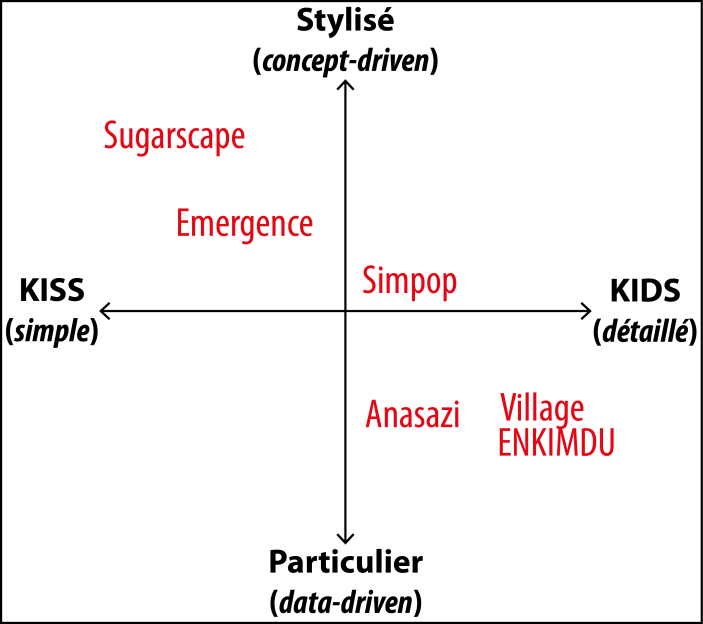
\includegraphics[width=.725\linewidth]{img/modelographie_fer-a-cheval.png}
	\caption[Une \og classification des approches de modélisation\fg{} de modèles géographiques.]{Une \og classification des approches de modélisation\fg{} de modèles géographiques, mobilisée pour une approche \og modélographique\fg{}.
	Tiré de \textcite[Figure 1]{schmitt_modelographie_2013}}
	\label{fig:modelographie}
\end{figure}


\paragraph{Origine de la trajectoire.}

La définition du point d'origine d'un modèle dans ce référentiel est plus difficile car éminemment subjective.
Selon le point de vue de celui qui positionnera le modèle, qu'il participe ou non à sa construction, la position peut ainsi assez largement varier.
On peut le montrer en s'appuyant sur un exercice qui avait réalisé à la fin du projet TransMonDyn, où un groupe de travail avait cherché à mener une \og TransModélographie\fg{}, c'est-à-dire une comparaison systématique des différents modèles construits au sein du projet.
Pour mener ce travail, nous avions commencé par présenter notre démarche aux différents participants du projet, et particulièrement en proposant une classification \og naïve\fg{} des modèles de chacun (\cref{fig:transmodelographie})

\begin{figure}[H]
	\centering
	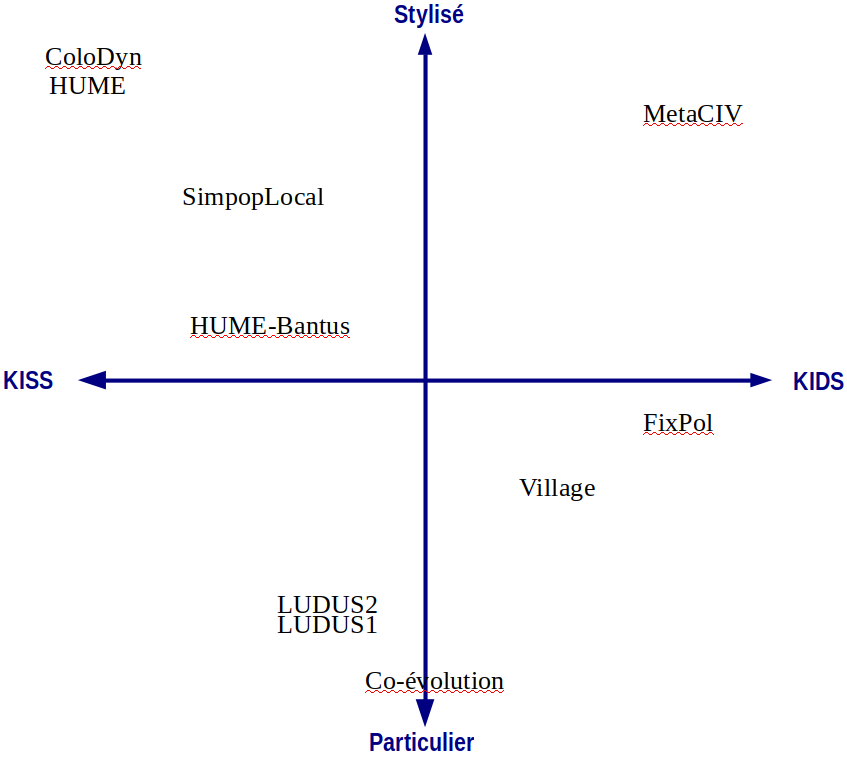
\includegraphics[width=\linewidth]{img/transmodelographie.png}
	\caption[Une proposition de \og TransModélographie\fg{}.]{Une proposition de \og TransModélographie\fg{}.\\
	Figure issue d'une communication à un séminaire interne du projet TransMonDyn à Tours, Octobre 2014, par Robin \textsc{Cura}, Hélène \textsc{Mathian} et Clara \textsc{Schmitt}.\\
	\textit{N.B. : Le modèle \og FixPol\fg{} (fixation et polarisation) est un ancien nom de SimFeodal.}}
	\label{fig:transmodelographie}
\end{figure}

À la suite de cette présentation, nous avons demandé aux participants de remplir un questionnaire\footnote{
	Toujours visible à cette adresse : \href{http://193.55.107.5/html/limesurvey/index.php/647837?lang=fr}{http://193.55.107.5/html/limesurvey/index.php/647837}
} visant justement à décrire, selon leur point de vue, le positionnement du modèle auquel ils participaient.
Faute de temps, ce projet n'a pas pu être mené à son terme, mais suite au dépouillement des premières réponses, nous avions noté la forte hétérogénéité des descriptions d'un même modèle, selon le rôle de l'intervenant (thématicien, modélisateur), mais aussi au sein de chaque rôle.
Les modèles ne changeaient pas réellement de cadran, mais en leur sein, la position déclarée par chacun variait fortement.

La définition du point d'origine de la trajectoire de SimFeodal est donc très subjective.
Par cohérence, je repartirai du positionnement affecté lors de cet expérience de \og TransModélographie\fg{}, ce qui correspond à un modèle résolument KIDS, mais situé dans un entre-deux entre le particulier et le stylisé (voir la position du modèle FixPol dans la \cref{fig:transmodelographie}). 

\paragraph{Qualifier la trajectoire de SimFeodal : l'exemple de la modélisation des seigneurs.}

De la même manière qu'il est difficile de définir l'origine du modèle, la caractérisation de sa trajectoire est un exercice périlleux.
En effet, un modèle peut présenter des composantes hétérogènes, c'est-à-dire que la description de tel mécanisme peut être très détaillée alors qu'un autre sera plus simple.
De même, le comportement d'un type d'agent peut être très stylisé quand celui d'un autre sera entièrement guidé par des données.

Dans le cas de SimFeodal, je prendrai alors l'exemple d'un mécanisme qui a fortement évolué durant le cycle de vie du modèle et a occupé une large part des discussions collectives : la modélisation des seigneurs, et notamment les mécanismes liés à la mise en place de réseaux de lignages seigneuriaux.
Lors de la réalisation du modèle conceptuel (visible dans \textcite[fig. 13.1, p. 297]{tannier_ontologie_2014}), il avait été décidé de différencier les seigneurs laïcs des seigneurs monastiques, dont on sait empiriquement que les logiques de constitution de lignages par le patrimoine, le don et la vassalité ne sont pas les mêmes.

\subparagraph{Origine - Étape 1.}Dans les premières versions du modèle implémenté, il y avait donc des agents de type \og seigneur laïque\fg{}, dotés de mécanismes proches de ceux des \og seigneurs\fg{} dans le modèle actuel (\hl{ref chap 2}).
Les agents \og seigneurs monastiques\fg{} étaient prévus mais il avait été choisi de commencer l'implémentation de manière incrémentale, en privilégiant d'abord d'autres agents.

\subparagraph{Étape 2.}Au fur et à mesure du développement du modèle, alors que certains types d'agents voyaient leurs mécanismes se complexifier dans une logique itérative, le modèle a atteint un premier stade de maturité et produit des résultats prometteurs.
Il a alors été choisi, par les thématiciens notamment, de délaisser la distinction entre seigneurs laïcs et seigneurs monastiques, ces derniers étant moins nombreux et représentatifs de la période.
Les seigneurs monastiques ont donc été enlevés du modèle conceptuel, qui n'a plus alors distingué que des \og seigneurs\fg{}, sans particularisation de type.
SimFeodal est ainsi progressé dans l'axe particulier-stylisé, en approchant plus d'une situation intermédiaire.

\subparagraph{Étape 3.}Quelques versions plus tard, alors que les dynamiques reproduites par le modèle devenaient plus satisfaisantes, nous avons voulu re-complexifier les mécanismes liés aux seigneurs.
La dimension polarisation était ainsi plutôt correcte, mais la hiérarchie des châteaux et des seigneurs était trop uniforme.
Pour faire apparaître une hiérarchisation plus forte et surtout pouvoir mieux l'observer, nous avons ajouté des indicateurs de sortie relatifs à la vassalité des seigneurs, et nous avons aussi adapté les mécanismes de dons de zones de prélèvement et de châteaux.
L'objectif était de reproduire le fait stylisé qui montre que les seigneurs distribuaient une partie de leurs possessions à des seigneurs de moindre importance en échange de loyauté, et donc de la mise en place de liens de vassalité.
De plus, pour que les réseaux de vassalité ainsi constitués aient une cohérence empirique, les seigneurs vérifiaient les liens des récipiendaires potentiels des dons : étaient écartés tous les petits seigneurs ayant, par succession de liens, des relations avec un autre grand seigneur.
Les lignages seigneuriaux prenaient ainsi la forme de deux arbres hiérarchiques, un grand seigneur concurrent étant à la tête de chaque arbre, dont nous pouvions alors mesurer le degré, le diamètre, la somme des puissances, etc.
Avec ces modifications, la trajectoire du modèle a d'une part été particularisé (axe Stylisé-Particulier), et d'autre part complexifié (axe KISS-KIDS).

\subparagraph{Étape 4.}La concentration, en termes de modélisation, s'est ensuite portée à nouveau sur la polarisation et la hiérarchisation du peuplement, notamment en introduisant le concept de l'agent \og pole d'attraction\fg{}, composé d'agents-attracteurs, qui permettait de réduire la complexité du modèle via ce type d'agent générique alors qu'auparavant, chaque type d'attracteur avait ses propres logiques.
Ce faisant, nous avons peu à peu accordé de moins en moins d'intérêt à l'évaluation visuelle de ces lignages seigneuriaux, jusqu'à ce qu'ils ne soient plus jamais pris en compte dans l'évaluation.
Pour acter cette évolution, dans la version 6 de SimFeodal (voir \hl{chap 3, tableau 3.1}), les thématiciens ont, d'eux-mêmes, suggéré de supprimer toute logique de constitution de réseau de vassalité : les dons des seigneurs sont désormais, comme décrit dans le \hl{chapitre 2}, effectués sans aucune distinction d'appartenance à un réseau seigneurial.
C'est maintenant une logique plus spatiale, liée à la distance entre les petits seigneurs, qui conditionne les potentiels récipiendaires de dons.
Cette suppression de distinction a ainsi donné une trajectoire inverse à la précédente dans le référentiel du fer à cheval : le modèle redevenait plus stylisé et moins descriptif.
Sur l'aspect seigneurial, le modèle devenait même plus stylisé et simple qu'il ne l'avait jamais été au cours de sa construction.

La \cref{fig:trajectoire-simfeodal} reprend graphiquement ces étapes, qui sont spécifiques au cas de la modélisation des seigneurs dans SimFeodal, mais permettent toutefois d'illustrer plus généralement la trajectoire d'ensemble du modèle.
En premier lieu, on peut noter que cette trajectoire ne s'inscrit pas dans les formes \og en fer à cheval\fg{} présentées par \textcite{banos2013modeliser} : les étapes intermédiaires ont \og déplacé\fg{} le modèle dans potentiellement toutes les directions, sans respecter une forme spécifique.
En second lieu, remarquons que SimFeodal, que je présente depuis l'introduction générale comme un modèle descriptif et exploratoire, ne semble plus si ancré dans l'approche KIDS dans sa version actuelle.

\begin{figure}[H]
	\centering
	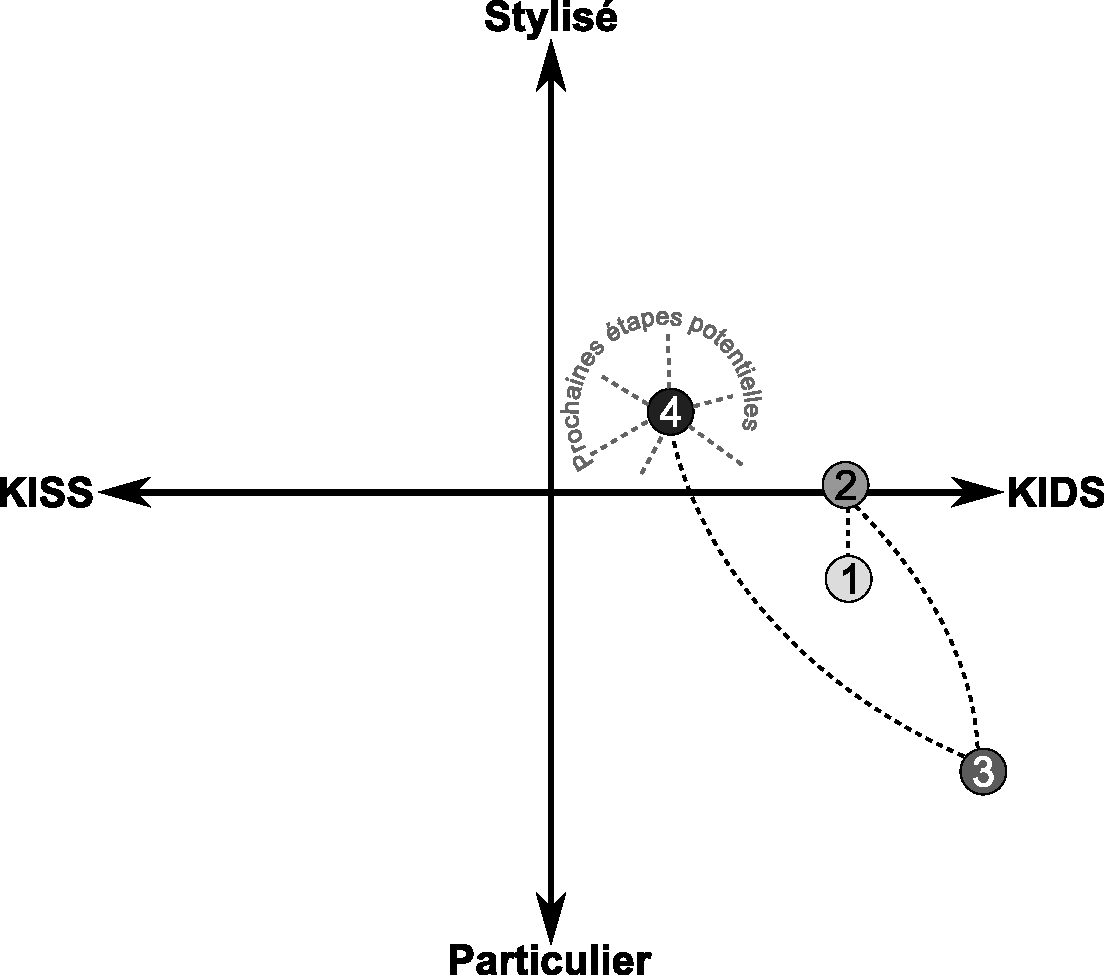
\includegraphics[width=.8\linewidth]{img/trajectoire_simfeodal.pdf}
	\caption[La trajectoire du modèle SimFeodal, dans le \og fer à cheval\fg{} de \textcite{banos2013modeliser}.]{La trajectoire du modèle SimFeodal, dans le \og fer à cheval\fg{} de \textcite{banos2013modeliser}.\\
	\textit{N.B.: cette trajectoire correspond à la position des mécanismes liés aux seigneurs dans le modèle.}}
	\label{fig:trajectoire-simfeodal}
\end{figure}

Il me semble que ces deux éléments peuvent s'expliquer par la nature de SimFeodal et de sa co-construction, qui est plus exploratoire et abductive que véritablement descriptive.
On peut ainsi noter des allers-retours fréquents entre augmentation et diminution de la complexité (axe KISS-KIDS) dans l'historique de développement du modèle.
Une partie de ces évolutions sont prévues dans la démarche KIDS \autocite{edmonds_kiss_2005}, qui vise à débuter par un modèle \og complexe\fg{}, descriptif, qui sera ensuite progressivement rendu plus simple si cela n'en diminue pas l'utilité.
La \og simplification\fg{} de SimFeodal s'inscrit donc nettement dans cette démarche.
La complexification de certains agents et mécanismes va pourtant à l'encontre de cette logique, et \textit{a posteriori}, j'aurais tendance à ne caractériser SimFeodal que comme un modèle exploratoire, sans le positionner véritablement sur l'axe KISS-KIDS, sinon en explicitant qu'on ne cherche pas particulièrement à ce que ce modèle soit KISS.

Ce sont avant tout les envies du groupe de travail qui guident le développement du modèle, influencées par les résultats successifs du modèle et par leur exploration.
Ces envies varient, s'accompagnent d'abandon de questionnements initiaux et de nouvelles questions, peuvent évoluer en sens inverse des choix passés, voire correspondre à de véritables \og retours en arrière\fg{} comme dans le cas des lignages seigneuriaux, abandonnés après avoir été très spécifiés.
SimFeodal est un modèle complexe, et sa trajectoire l'est aussi.
Cette trajectoire peut sembler irréfléchie et inexplicable, mais résulte en fait des multiples interactions entre les concepteurs de SimFeodal, et n'est que la matérialisation du processus abductif qui a guidé sa co-construction de SimFeodal.
À l'instar d'un mouvement brownien, la trajectoire de SimFeodal pourrait être modélisée par une marche aléatoire, et comme celle-ci, convergerait, à long terme, vers une exploration complète des possibilités de modélisation de ces dynamiques spatio-temporelles.

\subsection{Conclusion : Modéliser avec et pour les autres.}

Dans cette sous-partie, dédiée à un retour sur le processus de modélisation effectivement mené autour de SimFeodal, nous avons montré que le modèle, en tant qu'outil informatique, a constitué un support à la discussion interdisciplinaire et à l'explicitation des hypothèses et connaissances plus qu'à véritablement évaluer la capacité de ces hypothèses à reproduire les dynamiques empiriques de polarisation, de hiérarchisation et de fixation du peuplement.
La construction de SimFeodal n'a pas été trans-disciplinaire, dans le sens où les connaissances et compétences propres de chacun des participants ont été mutualisées dans les tâches qui y correspondaient le mieux, plutôt que de laisser chacun réaliser \og un peu de tout\fg{}.
De la même manière qu'on ne peut acquérir une connaissance thématique approfondie d'un sujet complètement inconnu en quelques années, on ne peut pas non plus acquérir les compétences techniques avancées nécessaires à l'implémentation de modèles de simulation complexes et détaillés.

Pour autant, je crois qu'on peut tout de même caractériser cette construction interdisciplinaire et collective comme une co-construction, car chacun est intervenu, à mesure de ses possibilités, sur chacune des étapes de la construction et de l'évaluation du modèle.
Ces interventions ont été de formes diverses, depuis la conception algorithmique des mécanismes jusqu'à leur implémentation technique, depuis leur validation interne par relecture du code jusqu'à leur validation externe par discussion et explicitation en groupe.
Il résulte de cette co-construction un modèle à la trajectoire chaotique, faite de fréquents allers-retours, et au positionnement final (et initial) difficile à caractériser tant ses composantes sont hétérogènes.
L'état \og final\fg{} de SimFeodal tout autant que son évolution, me paraissent inhérents au mode de co-construction résolument exploratoire qui a été suivi, le modèle servant alors d'outil de facilitation de mise en œuvre du processus abductif qui en résulte.

La satisfaction collective qui ressort de cette expérience de modélisation co-construite me paraît autant due à la volonté de chaque participant de s'inscrire pleinement dans cette expérience interdisciplinaire, d'accepter de passer outre les habitudes disciplinaires, qu'à l'horizontalité du processus et au temps long qui y a été consacré par chacun.

%\subsection{Construire et utiliser un modèle, deux approches et positions différentes}
%\paragraph{Modèle comme finalité, modèle comme apprentissage.}
%
%- On ressort l'argumentaire léna-esque habituel : enrichissement du à la formalisation et donc à l'explicitation.
%-> En plus, apport de l'implémentation et de l'évaluation : il faut trancher, il faut (parfois) quantifier, 

%\paragraph{Créateur et utilisateur : comment concilier des intérêts antagonistes ?}
%
%- attaquer par visions classiquement opposées du thématicien demandant détail et de l'informaticien-modélisateur cherchant parsimonie.
%- Solution optimale est forcément intermédiaire : approche SimFeodal : pas linéaire, mais tout de même du détail vers la parsimonie.
%- Opposée à approche inverse cf. RIN ATP (publi ?) de multi-modelling, = commencer par le plus simple et complexifier jusqu'à atteindre satisfaction des thématiciens

%\paragraph{Des gains, certes, mais pour qui ?}
%
%- Question principale : quelle discipline/champ scientifique veut-on faire avancer ?
%-> objectif théorique d'un projet interdisciplinaire : chacune des disciplines
%
%\paragraph{Conclusion : Modéliser avec et pour les autres.}
%- rubber duck, \og gardien de la vérité éprouvée\fg{}, 
%- Objectifs collectifs + objectifs individuels pour chacun

\section*{Conclusion}
\addcontentsline{toc}{section}{\protect\numberline{}Conclusion}

Ce chapitre \og pré-conclusif\fg{} a présenté deux retours réflexifs, assez isolés au premier regard, sur la spécificité de l'exploration de données de simulation et sur les modalités du processus de co-construction mis en œuvre dans le cadre de la construction et de l'évaluation de SimFeodal.
Chacune de ces sous-parties a déjà donné lieu à une conclusion intermédiaire, et je ne reviendrai ici que sur leur complémentarité.

Que ce soit sur le plan méthodologique de l'exploration de données issues de simulation, ou sur le plan conceptuel de la construction de modèle, l'élaboration d'une démarche exploratoire ressort comme un moyen fonctionnel de favoriser l'interdisciplinarité.
Cette démarche peut pour cela être bâtie autour d'un objet commun -- car partagé -- et neutre -- car à l'interface entre les disciplines --. 
L'objet commune que constitue le modèle et les données qu'il produit permettent de faire en sorte que le processus de modélisation ne soit pas qu'une expérience de pensée.
Cet objet matérialisé, parce qu'il peut être exploré, guide l'expérience collective et constitue ainsi une interface commune support au dialogue, en laissant l'exploration guider ce dialogue.

C'est en cela que la démarche mise en place autour de la construction et de l'évaluation peut être considérée comme facilitant la \og mise en situation d'étonnement\fg{} \autocite[241]{banos2005voie}.
L'exploration des hypothèses thématiques, par le modèle, et du modèle, par ses sorties, stimulent ainsi le cheminement abductif qui permet de dépasser les \textit{a priori} et implicites disciplinaires et d'aboutir à la réalisation d'un modèle utile à tous ses concepteurs.
